% Options for packages loaded elsewhere
\PassOptionsToPackage{unicode}{hyperref}
\PassOptionsToPackage{hyphens}{url}
\PassOptionsToPackage{dvipsnames,svgnames,x11names}{xcolor}
%
\documentclass[
]{krantz}
\usepackage{amsmath,amssymb}
\usepackage{iftex}
\ifPDFTeX
  \usepackage[T1]{fontenc}
  \usepackage[utf8]{inputenc}
  \usepackage{textcomp} % provide euro and other symbols
\else % if luatex or xetex
  \usepackage{unicode-math} % this also loads fontspec
  \defaultfontfeatures{Scale=MatchLowercase}
  \defaultfontfeatures[\rmfamily]{Ligatures=TeX,Scale=1}
\fi
\usepackage{lmodern}
\ifPDFTeX\else
  % xetex/luatex font selection
\fi
% Use upquote if available, for straight quotes in verbatim environments
\IfFileExists{upquote.sty}{\usepackage{upquote}}{}
\IfFileExists{microtype.sty}{% use microtype if available
  \usepackage[]{microtype}
  \UseMicrotypeSet[protrusion]{basicmath} % disable protrusion for tt fonts
}{}
\makeatletter
\@ifundefined{KOMAClassName}{% if non-KOMA class
  \IfFileExists{parskip.sty}{%
    \usepackage{parskip}
  }{% else
    \setlength{\parindent}{0pt}
    \setlength{\parskip}{6pt plus 2pt minus 1pt}}
}{% if KOMA class
  \KOMAoptions{parskip=half}}
\makeatother
\usepackage{xcolor}
\usepackage{color}
\usepackage{fancyvrb}
\newcommand{\VerbBar}{|}
\newcommand{\VERB}{\Verb[commandchars=\\\{\}]}
\DefineVerbatimEnvironment{Highlighting}{Verbatim}{commandchars=\\\{\}}
% Add ',fontsize=\small' for more characters per line
\usepackage{framed}
\definecolor{shadecolor}{RGB}{248,248,248}
\newenvironment{Shaded}{\begin{snugshade}}{\end{snugshade}}
\newcommand{\AlertTok}[1]{\textcolor[rgb]{0.33,0.33,0.33}{#1}}
\newcommand{\AnnotationTok}[1]{\textcolor[rgb]{0.37,0.37,0.37}{\textbf{\textit{#1}}}}
\newcommand{\AttributeTok}[1]{\textcolor[rgb]{0.27,0.27,0.27}{#1}}
\newcommand{\BaseNTok}[1]{\textcolor[rgb]{0.06,0.06,0.06}{#1}}
\newcommand{\BuiltInTok}[1]{#1}
\newcommand{\CharTok}[1]{\textcolor[rgb]{0.5,0.5,0.5}{#1}}
\newcommand{\CommentTok}[1]{\textcolor[rgb]{0.37,0.37,0.37}{\textit{#1}}}
\newcommand{\CommentVarTok}[1]{\textcolor[rgb]{0.37,0.37,0.37}{\textbf{\textit{#1}}}}
\newcommand{\ConstantTok}[1]{\textcolor[rgb]{0.37,0.37,0.37}{#1}}
\newcommand{\ControlFlowTok}[1]{\textcolor[rgb]{0.27,0.27,0.27}{\textbf{#1}}}
\newcommand{\DataTypeTok}[1]{\textcolor[rgb]{0.27,0.27,0.27}{#1}}
\newcommand{\DecValTok}[1]{\textcolor[rgb]{0.06,0.06,0.06}{#1}}
\newcommand{\DocumentationTok}[1]{\textcolor[rgb]{0.37,0.37,0.37}{\textbf{\textit{#1}}}}
\newcommand{\ErrorTok}[1]{\textcolor[rgb]{0.14,0.14,0.14}{\textbf{#1}}}
\newcommand{\ExtensionTok}[1]{#1}
\newcommand{\FloatTok}[1]{\textcolor[rgb]{0.06,0.06,0.06}{#1}}
\newcommand{\FunctionTok}[1]{\textcolor[rgb]{0.27,0.27,0.27}{\textbf{#1}}}
\newcommand{\ImportTok}[1]{#1}
\newcommand{\InformationTok}[1]{\textcolor[rgb]{0.37,0.37,0.37}{\textbf{\textit{#1}}}}
\newcommand{\KeywordTok}[1]{\textcolor[rgb]{0.27,0.27,0.27}{\textbf{#1}}}
\newcommand{\NormalTok}[1]{#1}
\newcommand{\OperatorTok}[1]{\textcolor[rgb]{0.43,0.43,0.43}{\textbf{#1}}}
\newcommand{\OtherTok}[1]{\textcolor[rgb]{0.37,0.37,0.37}{#1}}
\newcommand{\PreprocessorTok}[1]{\textcolor[rgb]{0.37,0.37,0.37}{\textit{#1}}}
\newcommand{\RegionMarkerTok}[1]{#1}
\newcommand{\SpecialCharTok}[1]{\textcolor[rgb]{0.43,0.43,0.43}{\textbf{#1}}}
\newcommand{\SpecialStringTok}[1]{\textcolor[rgb]{0.5,0.5,0.5}{#1}}
\newcommand{\StringTok}[1]{\textcolor[rgb]{0.5,0.5,0.5}{#1}}
\newcommand{\VariableTok}[1]{\textcolor[rgb]{0,0,0}{#1}}
\newcommand{\VerbatimStringTok}[1]{\textcolor[rgb]{0.5,0.5,0.5}{#1}}
\newcommand{\WarningTok}[1]{\textcolor[rgb]{0.37,0.37,0.37}{\textbf{\textit{#1}}}}
\usepackage{longtable,booktabs,array}
\usepackage{calc} % for calculating minipage widths
% Correct order of tables after \paragraph or \subparagraph
\usepackage{etoolbox}
\makeatletter
\patchcmd\longtable{\par}{\if@noskipsec\mbox{}\fi\par}{}{}
\makeatother
% Allow footnotes in longtable head/foot
\IfFileExists{footnotehyper.sty}{\usepackage{footnotehyper}}{\usepackage{footnote}}
\makesavenoteenv{longtable}
\usepackage{graphicx}
\makeatletter
\def\maxwidth{\ifdim\Gin@nat@width>\linewidth\linewidth\else\Gin@nat@width\fi}
\def\maxheight{\ifdim\Gin@nat@height>\textheight\textheight\else\Gin@nat@height\fi}
\makeatother
% Scale images if necessary, so that they will not overflow the page
% margins by default, and it is still possible to overwrite the defaults
% using explicit options in \includegraphics[width, height, ...]{}
\setkeys{Gin}{width=\maxwidth,height=\maxheight,keepaspectratio}
% Set default figure placement to htbp
\makeatletter
\def\fps@figure{htbp}
\makeatother
\setlength{\emergencystretch}{3em} % prevent overfull lines
\providecommand{\tightlist}{%
  \setlength{\itemsep}{0pt}\setlength{\parskip}{0pt}}
\setcounter{secnumdepth}{5}
\usepackage{booktabs}
\usepackage{longtable}
\usepackage[bf,singlelinecheck=off]{caption}

\usepackage{framed,color}
\definecolor{shadecolor}{RGB}{248,248,248}

\renewcommand{\textfraction}{0.05}
\renewcommand{\topfraction}{0.8}
\renewcommand{\bottomfraction}{0.8}
\renewcommand{\floatpagefraction}{0.75}

\renewenvironment{quote}{\begin{VF}}{\end{VF}}
\let\oldhref\href
\renewcommand{\href}[2]{#2\footnote{\url{#1}}}

\makeatletter
\newenvironment{kframe}{%
\medskip{}
\setlength{\fboxsep}{.8em}
 \def\at@end@of@kframe{}%
 \ifinner\ifhmode%
  \def\at@end@of@kframe{\end{minipage}}%
  \begin{minipage}{\columnwidth}%
 \fi\fi%
 \def\FrameCommand##1{\hskip\@totalleftmargin \hskip-\fboxsep
 \colorbox{shadecolor}{##1}\hskip-\fboxsep
     % There is no \\@totalrightmargin, so:
     \hskip-\linewidth \hskip-\@totalleftmargin \hskip\columnwidth}%
 \MakeFramed {\advance\hsize-\width
   \@totalleftmargin\z@ \linewidth\hsize
   \@setminipage}}%
 {\par\unskip\endMakeFramed%
 \at@end@of@kframe}
\makeatother

\renewenvironment{Shaded}{\begin{kframe}}{\end{kframe}}

\newenvironment{rmdblock}[1]
  {
  \begin{itemize}
  \renewcommand{\labelitemi}{
    \raisebox{-.7\height}[0pt][0pt]{
      {\setkeys{Gin}{width=3em,keepaspectratio}\includegraphics{images/#1}}
    }
  }
  \setlength{\fboxsep}{1em}
  \begin{kframe}
  \item
  }
  {
  \end{kframe}
  \end{itemize}
  }
\newenvironment{rmdnote}
  {\begin{rmdblock}{note}}
  {\end{rmdblock}}
\newenvironment{rmdcaution}
  {\begin{rmdblock}{caution}}
  {\end{rmdblock}}
\newenvironment{rmdimportant}
  {\begin{rmdblock}{important}}
  {\end{rmdblock}}
\newenvironment{rmdtip}
  {\begin{rmdblock}{tip}}
  {\end{rmdblock}}
\newenvironment{rmdwarning}
  {\begin{rmdblock}{warning}}
  {\end{rmdblock}}
\newenvironment{rmdreminder}
  {\begin{rmdblock}{reminder}}
  {\end{rmdblock}}
\newenvironment{rmdinfo}
  {\begin{rmdblock}{info}}
  {\end{rmdblock}}
  
\usepackage{makeidx}
\makeindex

\urlstyle{tt}

\usepackage{amsthm}
\makeatletter
\def\thm@space@setup{%
  \thm@preskip=8pt plus 2pt minus 4pt
  \thm@postskip=\thm@preskip
}
\makeatother

\frontmatter
\ifLuaTeX
  \usepackage{selnolig}  % disable illegal ligatures
\fi
\usepackage[]{natbib}
\bibliographystyle{apalike}
\IfFileExists{bookmark.sty}{\usepackage{bookmark}}{\usepackage{hyperref}}
\IfFileExists{xurl.sty}{\usepackage{xurl}}{} % add URL line breaks if available
\urlstyle{same}
\hypersetup{
  pdftitle={Notes on Network Science},
  pdfauthor={Hongtao Hao},
  colorlinks=true,
  linkcolor={Maroon},
  filecolor={Maroon},
  citecolor={Blue},
  urlcolor={Blue},
  pdfcreator={LaTeX via pandoc}}

\title{Notes on Network Science}
\author{Hongtao Hao}
\date{2025-10-17}

\begin{document}
\maketitle

{
\hypersetup{linkcolor=}
\setcounter{tocdepth}{2}
\tableofcontents
}
\hypertarget{welcome}{%
\chapter*{Welcome}\label{welcome}}


This online book is largely inspired by Professor \href{https://yongyeol.com/}{Yong-Yeol (``YY'') Ahn}'s online class of \href{http://yongyeol.com/teaching/2020SP_netsci_syllabus.pdf}{INFO I606 \emph{Network Science}} at Indiana University Bloomington, and the \href{http://networksciencebook.com/}{\emph{Network Science}} book by \href{https://barabasi.com/}{Albert-László Barabási}. I am deeply grateful to Professor YY Ahn for allowing me to attend the online course and to Professor Barabási for generously making his book available to everyone online. Without their help, this project is impossible.

This book has several custom blocks:

\begin{rmdnote}
This is a note, a general notice.
\end{rmdnote}

\begin{rmdreminder}
This is a reminder, usually just to remind myself of something I do not understand yet.
\end{rmdreminder}

\begin{rmdtip}
This is a tip, which helps you to understand a concept or memorize a formula.
\end{rmdtip}

\begin{rmdcaution}
This is a caution, to inform you, for example, an error in publications.
\end{rmdcaution}

\begin{rmdimportant}
This is an importance note. It tells you something you should consider when understanding a concept, for example, when scholars disagree.
\end{rmdimportant}

This website is built with \href{https://bookdown.org/}{Bookdown} and deployed by \href{https://www.netlify.com/}{Netlify}. You can find the full source of this project at \url{https://github.com/hongtaoh/netsci-notes}.

\includegraphics{images/license.png}

This book is licensed under the \href{http://creativecommons.org/licenses/by-nc-sa/4.0/}{Creative Commons Attribution-NonCommercial-ShareAlike 4.0 International License}.

If you notice any errors, including typos and mistakes in math formulas, you are welcome to contribute to the project by clicking the ``Editing'' button on the upper-left of this online book (shown below). You will be directed to fork this project before suggesting changes.

\begin{center}\includegraphics[width=0.45\linewidth]{images/edit} \end{center}

\mainmatter

\hypertarget{intro}{%
\chapter{Introduction to Network Science}\label{intro}}

We are going to dive into the field of network science. To learn a new subject, it's always beneficial to learn a little bit about it's history, definition, and significance. These will be the focus of this Chapter.

\hypertarget{intro-to-networks}{%
\section{Intro to networks}\label{intro-to-networks}}

\begin{rmdnote}
The following is not originally from me, but my notes from reading \href{http://networksciencebook.com/}{\emph{Network Science}} (Ch. 1.1-1.4) by \href{https://barabasi.com/}{Albert-László Barabási}. Notes are accompanied by my explanations.
\end{rmdnote}

\hypertarget{networks-and-complex-systems}{%
\subsection{Networks and complex systems}\label{networks-and-complex-systems}}

A system is a \textbf{complex system} when we cannot know its collective behavior by simply understanding each individual component within it. To really understand complex systems, we need to gain a deeper understanding of \textbf{networks} behind these syetems.

Despite that networks are different in size, nature, function, etc., they are orgnized by a common set of rules. That's why we are able to study them.

\hypertarget{driving-forces-behind-network-sciences-emerging-as-a-discipline}{%
\subsection{Driving forces behind network science's emerging as a discipline}\label{driving-forces-behind-network-sciences-emerging-as-a-discipline}}

Networks are not new. They have been studied by scientists in other disciplines for centuries. But why did network science become a discipline in the 21st centuary? There are two driving forces behind it:

\begin{enumerate}
\def\labelenumi{\arabic{enumi}.}
\tightlist
\item
  \textbf{The emergence of network maps}
\end{enumerate}

Mapping interactions in networks requires we keep track of huge amounts of data. This was not readily available until the start of the 21st century.

\begin{enumerate}
\def\labelenumi{\arabic{enumi}.}
\setcounter{enumi}{1}
\tightlist
\item
  \textbf{The universality of network characteristics}
\end{enumerate}

In the past, people knew different networks, but they didn't realize that as different as these networks are, they are indeed similar and share the same principles.

\hypertarget{key-characteristics-of-network-science}{%
\subsection{Key characteristics of network science}\label{key-characteristics-of-network-science}}

Network science has the following key characteristics:

\begin{itemize}
\tightlist
\item
  \textbf{Interdisciplinary}
\end{itemize}

Scientists in different disciplines working with networks have their own problems to solve and tasks to perform. However, some of their tasks share similarities, and a solution found in discipline A might turn out to be useful and important for discipline B as well.

\begin{itemize}
\tightlist
\item
  \textbf{Empirical, \& data driven}
\end{itemize}

Network science is empirical in nature. Every tool developed by network scientists should pass the test of data in real life and should offer people deeper insights about the network.

\begin{itemize}
\tightlist
\item
  \textbf{Quantitative and mathematical}
\end{itemize}

Network science has been borrowing the fromalism from \href{https://en.wikipedia.org/wiki/Graph_theory}{graph theory}, the conceptual framework from statistical physics, and concepts from engineering.

\begin{itemize}
\tightlist
\item
  \textbf{Computational}
\end{itemize}

Scientists of network science need to deal with a vast amount of data. They'll need to apply computational methods.

\hypertarget{definition-and-significance-of-networks}{%
\section{Definition and significance of networks}\label{definition-and-significance-of-networks}}

\begin{rmdnote}
The following came from the online course of \href{https://github.com/yy/netsci-course}{INFO 606} at Indiana University taught by Professor \href{https://yongyeol.com/}{Yong-Yoel (``YY'') Ahn}.
\end{rmdnote}

\hypertarget{what-is-a-network}{%
\subsection{What is a network}\label{what-is-a-network}}

A network is \textbf{a system of elements that are connected}. Those elements are called \textbf{nodes} or \textbf{vertices}, and the connections are called \textbf{links} or \textbf{edges}. Network science is all about \textbf{connections}.

There are two things that we care about in connections in a network: \textbf{structure}, and \textbf{dynamics}. Structure and dynamics might affect each other. Professor YY took Facebook activity as an example. Interpersonal interactions on and through facebook are governed by the structure of your friends you have on FB; On the other hand, if someone keeps posting things that iritate you, you might unfriend him or her, which will alter the structure of your online friends network.

I thought about international relationships. Relationships between countries vary: some are strong while others are weak. These structures definitely have an effect on the things going on between countries. Then, if a country does something that make another country, or other countries angry, for example, initiating a war, the original structure might witness drastic changes.

\hypertarget{why-should-we-care-about-networks}{%
\subsection{Why should we care about networks?}\label{why-should-we-care-about-networks}}

\hypertarget{understanding-individual-elements-is-far-from-enough.}{%
\subsubsection{Understanding individual elements is far from enough.}\label{understanding-individual-elements-is-far-from-enough.}}

Knowing about each neuron in a person's brain cannot gaurantee you can understand how a brain functions, or even rebuild a brain. To do these, we need to how elements interact.

\hypertarget{networks-are-everywhere.}{%
\subsubsection{Networks are everywhere.}\label{networks-are-everywhere.}}

Human body, Internet, electricity, food, forest, the universe, etc., all have networks in them.

Networks are omnipresent. Some networks are waiting for discovery and finding a new network itself can be a contribution. For example, professor YY and his colleagues found this \href{https://www.nature.com/articles/srep00196}{flavor network}.

Also, the fact that networks are everything mean they have huge influence on our lives. A prime example would be pandemics. A contagious disease won't stay locally anymore, thanks to the advancing global air transportation. The Coronavirus Disease 2019 (COVID-19) was first found in China and in only several months, it became a nightmare for every country in the world.

\hypertarget{networks-let-us-make-fun-analogies.}{%
\subsubsection{Networks let us make fun analogies.}\label{networks-let-us-make-fun-analogies.}}

Network thinking: everything is a system consisting of many individual elements that are connected and interact.

This thought help scientists make analogies and new discoveries. For example, in the 19th centuary, it led to probabilistic and statistical thinking.

Professor YY gave an example of this own. He was studying how hastags spread on Twitter. The goal was to predic viral hastags. Later, some other scientists applied this finding to human brain and published \href{https://www.sciencedirect.com/science/article/pii/S0896627315004742}{this paper}.

\hypertarget{think-for-yourself}{%
\subsection{Think for yourself}\label{think-for-yourself}}

Can you give an example of a network in your life?

\hypertarget{python-setup}{%
\section{Python setup}\label{python-setup}}

\begin{rmdnote}
The following is based on Professor YY's \href{https://github.com/yy/netsci-course/blob/master/m01-getready/python-setup.md}{tutorial on Python setup}.
\end{rmdnote}

Throughout this tutorial, we'll use \href{https://www.python.org/}{Python}. Specifically, we'll use the package called \href{https://networkx.github.io/documentation/stable/index.html}{Networkx}. Networkx is useful and handy in terms of calculating properties of networks but isn't always helpful for creating visualizations. To visualize networks, we'll use \href{https://gephi.org/}{Gephi}.

We'll be using \href{https://www.anaconda.com/products/individual}{Anaconda} to manage python packages. \href{https://jupyter.org/install.html}{Jupyter Notebook} will be where we write and run our python codes.

Don't worry if you don't know anything about any of them. I'll walk you through them now.

\hypertarget{anaconda}{%
\subsubsection{Anaconda}\label{anaconda}}

You can refer to \href{https://www.youtube.com/watch?v=YJC6ldI3hWk}{this video} to get a better understanding of why and how to use Anaconda.

To install Anaconda, go \href{https://www.anaconda.com/products/individual\#Downloads}{here} and choose the version for you. For MacOs, choose the ``Command Line Installer'' \textbf{only if you want to feel like a hacker}.

\hypertarget{if-you-dont-have-enough-storage}{%
\paragraph{If you don't have enough storage}\label{if-you-dont-have-enough-storage}}

The full Anaconda takes more than 3G of your storage. If storage is a problem for you, you can install the lightweight version of it: \href{https://docs.conda.io/en/latest/miniconda.html}{Miniconda}. You can look \href{https://stackoverflow.com/questions/45421163/anaconda-vs-miniconda}{here} to know more about the differences between the two. To put it simply, Anaconda comes with \href{https://docs.anaconda.com/anaconda/packages/py3.8_osx-64/}{a long list of packages} pre-installed, so you don't have to install each of them separately by yourself. However, you'll have to do so for Miniconda.

If you decide to use Miniconda for whatever reason, after installing it, open your \texttt{Terminal} and do the following (If you are using Anaconda, you don't need to). I am assuming that you are using a Mac:

\begin{Shaded}
\begin{Highlighting}[]
\ExtensionTok{conda} \AttributeTok{{-}{-}version} \CommentTok{\# To check whether the installation was successful}
\end{Highlighting}
\end{Shaded}

If the installation was successful, then do the following:

\begin{Shaded}
\begin{Highlighting}[]
\CommentTok{\# To download jupyter notebook, and jupyterlab:}
\ExtensionTok{conda}\NormalTok{ install }\AttributeTok{{-}c}\NormalTok{ conda{-}forge vega notebook jupyterlab }
\CommentTok{\# To download packages we\textquotesingle{}ll need to use later:}
\ExtensionTok{conda}\NormalTok{ install numpy scipy networkx jupyter }
\ExtensionTok{conda}\NormalTok{ install pandas matplotlib seaborn bokeh scikit{-}learn }
\end{Highlighting}
\end{Shaded}

Even if you are using Anaconda, sometimes you might need to use some packages that are not already installed and you'll need to install them by yourself. Simply run \texttt{conda\ install\ your-package-name}. Most of the packages could be installed that way. Of course, you can still use \texttt{pip} to download packages even if you are using Anaconda (or Miniconda). Run \texttt{pip\ your-package-name}.

\hypertarget{if-you-dont-want-to-use-either-anaconda-or-miniconda}{%
\paragraph{If you don't want to use either Anaconda or Miniconda}\label{if-you-dont-want-to-use-either-anaconda-or-miniconda}}

If your computer is running on a MacOS or a Linux system, then you can also use \texttt{pip} to install python packages. First, you need to download Python \href{https://www.python.org/downloads/}{here}. Then, go to \texttt{Terminal} and run the following code, which came from \href{https://github.com/yy/netsci-course/blob/master/m01-getready/python-setup.md}{Professor YY's tutorial}.

\begin{Shaded}
\begin{Highlighting}[]
\ExtensionTok{pip3}\NormalTok{ install numpy scipy networkx jupyter jupyterlab ipython }
\ExtensionTok{pip3}\NormalTok{ install pandas matplotlib seaborn bokeh scikit{-}learn}
\end{Highlighting}
\end{Shaded}

\hypertarget{jupyter-notebook}{%
\subsubsection{Jupyter Notebook}\label{jupyter-notebook}}

As Professor YY suggests, to gain a deeper understanding of Jupyter Notebook, you can watch \href{https://www.youtube.com/watch?v=HW29067qVWk}{this tutorial} and \href{https://www.youtube.com/watch?v=2eCHD6f_phE}{this demonstration}.

As the above two videos showed, to open jupyter notebook, you simply need to type \texttt{jupyter\ notebook} in your \texttt{Terminal}. It's quite straightforward. One trick you might need to know is that you can first go to the directory of your file, for example, \texttt{cd\ Desktop/netsci} and then run \texttt{jupyter\ notebook}. This way, you can use jupyter notebook right in the folder you want. This might save some of your time.

\hypertarget{jupyter-notebook-on-the-cloud}{%
\paragraph{Jupyter Notebook On the cloud}\label{jupyter-notebook-on-the-cloud}}

If you don't want to use jupyter notebook on your computer, you can try \href{https://colab.research.google.com/notebooks/intro.ipynb}{Google's Colab} which allows you to run python codes on the cloud.

\hypertarget{most-importantly-python}{%
\subsubsection{Most importantly, Python}\label{most-importantly-python}}

I haven't talked about Python, the most important tool we are going to use in this tutorial yet. I don't recommend you to attend a detailed python course now, since it's not necessary for this tutorial.

To get started with Python, read these two instructions:

\begin{enumerate}
\def\labelenumi{\arabic{enumi}.}
\tightlist
\item
  \href{https://docs.python.org/3.7/tutorial/introduction.html}{An Informal Introduction to Python}
\item
  \href{https://docs.python.org/3.7/tutorial/controlflow.html}{More Control Flow Tools}
\end{enumerate}

Do expect one, two, or even more days on these if you don't have any experience using Python before. Make sure that you understand most of the codes in the above two instructions before you begin. Open your \texttt{jupyter\ notebook} and try to implement the codes in the above two tutorials now.

\hypertarget{homework}{%
\section{Homework}\label{homework}}

\begin{rmdnote}
The following is based on Professor YY's \href{https://github.com/yy/netsci-course/blob/master/m01-getready/Python\%20Introduction\%20Assignment.ipynb}{Python Introduction Assignment}.
\end{rmdnote}

Create a notebook, name it as \texttt{python-setup}, and run the following codes:

\begin{Shaded}
\begin{Highlighting}[]
\ImportTok{import}\NormalTok{ numpy }\ImportTok{as}\NormalTok{ np }
\ImportTok{import}\NormalTok{ networks }\ImportTok{as}\NormalTok{ nx}
\ImportTok{import}\NormalTok{ matplotlib }\ImportTok{as}\NormalTok{ plt}
\OperatorTok{\%}\NormalTok{ matplotlib inline}
\end{Highlighting}
\end{Shaded}

If you have successfully downloaded Anaconda, you won't see any errors. If you do, go back and read \href{https://netsci.hongtaoh.com/python-setup.html}{the instructions} more carefully. Chances are that you might have missed some steps. Use Google or other search engines to look for answers to questions not discussed here.

Thanks.

\hypertarget{Graph}{%
\chapter{Graph Theory and Some Basic Concepts}\label{Graph}}

\begin{rmdnote}
The following is not originally from me, but my notes from reading \href{http://networksciencebook.com/}{\emph{Network Science}} (Ch. 2.1-2.3) by \href{https://barabasi.com/}{Albert-László Barabási}. Notes are accompanied by my explanations.
\end{rmdnote}

What is a network composed of? How is a network different from another one? In this chapter, we are going to study some very basic concepts of network science: size of a network, number of links, degree, average degree, degree distribution, and adjacency matrix.

\hypertarget{kuxf6nigsberg-bridge-problem-ch.-2.1}{%
\section{Königsberg bridge problem (Ch. 2.1)}\label{kuxf6nigsberg-bridge-problem-ch.-2.1}}

\begin{figure}

{\centering \includegraphics[width=0.7\linewidth]{./images/bridge} 

}

\caption{Leonhard Euler's drawing of the seven bridges in Königsberg, Image credit: beanz Magazine}\label{fig:unnamed-chunk-15}
\end{figure}

The above image is from \href{https://www.kidscodecs.com/7-bridges-konigsberg/}{\emph{beanz Magazine}}.

The challenge: Are you able to wall across all the seven bridges but cross each bridge only once? The starting and ending point is not specified.

Before reading on, I highly recommend you to try \href{https://www.mathsisfun.com/activity/seven-bridges-konigsberg.html}{this exercise} on \href{https://www.mathsisfun.com/}{mathsisfun.com} by yourself. Getting the answer from others won't help you learn it at the deepest level.

\begin{center}\rule{0.5\linewidth}{0.5pt}\end{center}

\textbf{Solution} to this challenge: if a path exists which allows a person to cross all the bridges but walk across each bridge only once, which is called a ``\textbf{Euler Path}'', the number of nodes having an odd number of bridges should be either zero or two. When there are two nodes having an odd number of bridges, i.e., having an odd degree (a point we'll learn later), one of the two nodes should be the starting point and the other the end point.

This remarkable discovery by Euler led to the development of a new branch in mathematics: \href{https://en.wikipedia.org/wiki/Graph_theory}{graph theory}.

\hypertarget{networks-and-graphs-ch.-2.2}{%
\section{Networks and graphs (Ch. 2.2)}\label{networks-and-graphs-ch.-2.2}}

The components in a network are called \textbf{nodes} or \textbf{vertices} and the direct connections between them are called \textbf{links} or \textbf{edges}. When we are describing a network in real life, it's better to use \textbf{networks}, \textbf{nodes}, and \textbf{links}, whereas \textbf{graphs}, \textbf{vertices}, and \textbf{edges} are mostly used for an abstract representation of networks. Some people do not care about these distinctions, though.

\textbf{\emph{N}}, meaning the \textbf{number of nodes}, is also called the \textbf{size of the network}. Nodes are labeled as \textbf{\emph{i}} = 1,2,3,\ldots, \emph{N}

\textbf{\emph{L}}, representing the \textbf{total number of links} in a network.

For an individual link, we may represent it as \((i, j)\). For example, (2,4) denotes the link connecting nodes 2 and 4.

Links can either be \textbf{directed} or \textbf{undirected}. If I make a phone call to you, then the link between us is from me to you. It is \textbf{directed}. If we are friends on social media, then this link is \textbf{undirected}.

A network is \textbf{directed} if all of its links are \textbf{directed}. If all of its links are \textbf{undirected}, then this network is an \textbf{undirected} network.

\hypertarget{degree-average-degree-and-degree-distribution-ch.-2.3}{%
\section{Degree, average degree, and degree distribution (Ch. 2.3)}\label{degree-average-degree-and-degree-distribution-ch.-2.3}}

\hypertarget{degree}{%
\subsection{Degree}\label{degree}}

The \textbf{degree} of a node is simply the number of links connecting it to other nodes.

\begin{Shaded}
\begin{Highlighting}[]
\FunctionTok{library}\NormalTok{(igraph)}
\FunctionTok{par}\NormalTok{(}\AttributeTok{mar =} \FunctionTok{c}\NormalTok{(}\DecValTok{1}\NormalTok{, }\DecValTok{1}\NormalTok{, }\DecValTok{1}\NormalTok{, }\DecValTok{1}\NormalTok{))}
\NormalTok{g1 }\OtherTok{\textless{}{-}} \FunctionTok{graph}\NormalTok{( }\AttributeTok{edges=}\FunctionTok{c}\NormalTok{(}\DecValTok{1}\NormalTok{,}\DecValTok{2}\NormalTok{, }\DecValTok{1}\NormalTok{,}\DecValTok{3}\NormalTok{, }\DecValTok{2}\NormalTok{,}\DecValTok{3}\NormalTok{, }\DecValTok{3}\NormalTok{,}\DecValTok{4}\NormalTok{), }\AttributeTok{n=}\DecValTok{4}\NormalTok{, }\AttributeTok{directed=}\ConstantTok{FALSE}\NormalTok{)}
\end{Highlighting}
\end{Shaded}

\begin{verbatim}
## Warning: `graph()` was deprecated in igraph 2.1.0.
## i Please use `make_graph()` instead.
## This warning is displayed once every 8 hours.
## Call `lifecycle::last_lifecycle_warnings()` to see where this warning was
## generated.
\end{verbatim}

\begin{Shaded}
\begin{Highlighting}[]
\FunctionTok{plot}\NormalTok{(g1)}
\end{Highlighting}
\end{Shaded}

\begin{figure}

{\centering 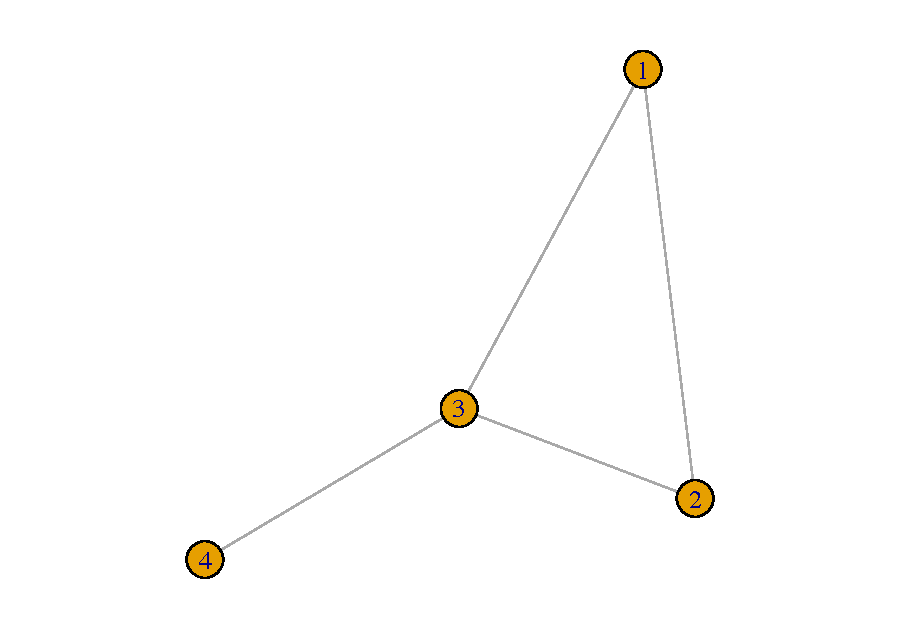
\includegraphics[width=0.9\linewidth]{netsci_files/figure-latex/nunit2-nodes-1} 

}

\caption{An undirected network for illustration.}\label{fig:nunit2-nodes}
\end{figure}

For example, in the above network, nodes 1, 2, and 4 have a degree of two. Node 3 has a degree of three.

For the \(i^{th}\) node in a network, we'll denote its degree as \(k_i\). Therefore, for the above network, \(k_1\)=\(k_2\)=\(k_4\)=2, \(k_3\)=3.

As mentioned above, the \textbf{total number of links} is denoted as \textbf{\emph{L}}. In an undirected network, it is easy to understand that \textbf{\emph{L}} should be half of the sum of all the node degrees. It should be halved because each link belongs to two nodes and therefore each is counted twice. We have:

\begin{equation} 
  L = \frac{1}{2} \sum_{i=1}^N k_i \label{eq:TotalLink}
\end{equation}

In the above network, \(L = 4\).

\hypertarget{average-degree}{%
\subsection{Average degree}\label{average-degree}}

\textbf{Average degree}, denoted as \(\langle k \rangle\) is simply the mean of all the node degrees in a network. For the network above (Figure \ref{fig:nunit2-nodes}), \(\langle k \rangle = \frac{1}{4} \cdot (k_1 + k_2 + k_3 + k_4) = \frac{1}{4} \cdot (2+2+3+1) = 2\). This means that on average, each node in the network has 2.25 links.

According to its definition, we know that \(\langle k \rangle\) = \(\frac{1}{N} \sum_{i=1}^N k_i\). Combined with Eq. \eqref{eq:TotalLink}, we have:

\begin{equation} 
  \langle k \rangle = \frac{2L}{N} \label{eq:AverageDegree}
\end{equation}

How can we understand this equation?

I would understand it this way: we are calculating the \textbf{average} degree, so the denominator will be \textbf{\emph{N}}, i.e., number of nodes, and the nominator will be the sum of all the nodes' number of links, which should be \(2L\) because each link is shared by two nodes.

The above equation Eq. \eqref{eq:AverageDegree} is for undirected networks. What about directed networks? Should we calculate their average degree the same way?

\begin{Shaded}
\begin{Highlighting}[]
\NormalTok{g2 }\OtherTok{\textless{}{-}} \FunctionTok{graph}\NormalTok{( }\AttributeTok{edges=}\FunctionTok{c}\NormalTok{(}\DecValTok{1}\NormalTok{,}\DecValTok{2}\NormalTok{, }\DecValTok{1}\NormalTok{,}\DecValTok{3}\NormalTok{, }\DecValTok{2}\NormalTok{,}\DecValTok{3}\NormalTok{, }\DecValTok{3}\NormalTok{,}\DecValTok{4}\NormalTok{), }\AttributeTok{n=}\DecValTok{4}\NormalTok{, }\AttributeTok{directed=}\ConstantTok{TRUE}\NormalTok{)}
\FunctionTok{par}\NormalTok{(}\AttributeTok{mar =} \FunctionTok{c}\NormalTok{(}\DecValTok{1}\NormalTok{, }\DecValTok{1}\NormalTok{, }\DecValTok{1}\NormalTok{, }\DecValTok{1}\NormalTok{))}
\FunctionTok{plot}\NormalTok{(g2)}
\end{Highlighting}
\end{Shaded}

\begin{figure}

{\centering 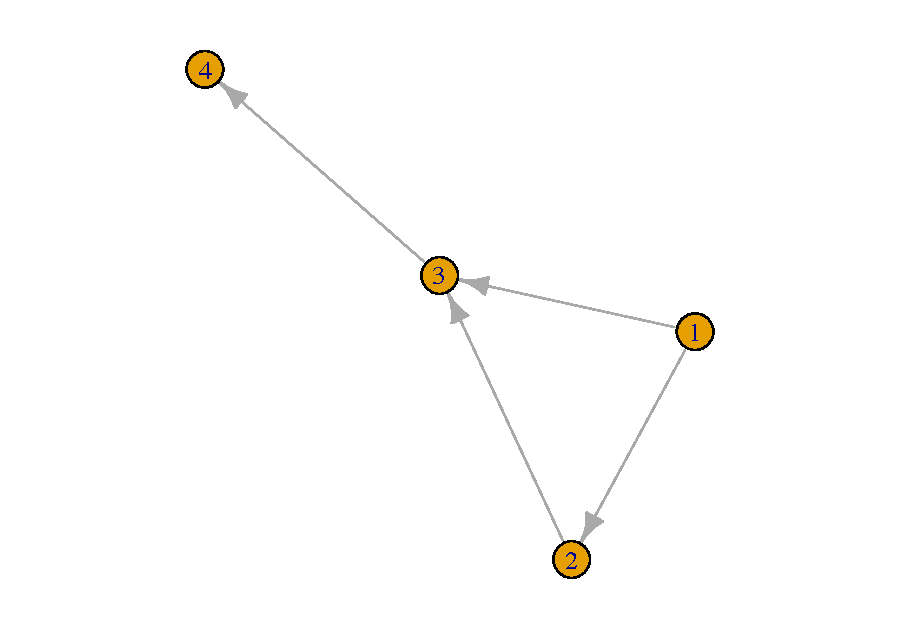
\includegraphics[width=0.9\linewidth]{netsci_files/figure-latex/nunit2-nodes-directed-1} 

}

\caption{A directed network for illustration.}\label{fig:nunit2-nodes-directed}
\end{figure}

Each link in the above network (\ref{fig:nunit2-nodes-directed}) is directed. If we calculate the network's average degree according to Eq. \eqref{eq:AverageDegree}, we will be losing information.

Therefore, we will distinguish between \textbf{incoming degree}, denoted as \(k_i^{in}\) and \textbf{outgoing degree}, denoted as \(k_i^{out}\). \(k_i^{in}\) means the number of links from other nodes pointing to node \(i\), and \(k_i^{out}\) means the number of links starting from node \(i\) and pointing to other nodes.

For a given node \(i\) in a directed network, its degree is the sum of incoming degree and outgoing degree. Therefore,

\begin{equation} 
  k_i = k_i^{in} + k_i^{out} \label{eq:degree-directed}
\end{equation}

And \textbf{\emph{L}}, the total number of links in a directed network, is:

\begin{equation}
  L = \sum_{i=1}^N k_i^{in} = \sum_{i=1}^N k_i^{out} \label{eq:total-links-directed}
\end{equation}

For a directed link between node \emph{i} and node \emph{j}, i.e., (\emph{i}, \emph{j}), it constitutes an \textbf{incoming degree} for one node, but an \textbf{outgoing degree} for the other. For example, in the network (\ref{fig:nunit2-nodes-directed}), (1,2) counts as an \textbf{incoming degree} for node 2, but an \textbf{outgoing degree} for node 1.

In fact, if we combine Eq. \eqref{eq:degree-directed} with Eq. \eqref{eq:total-links-directed}, we will know that Eq. \eqref{eq:total-links-directed} is equal to Eq. \eqref{eq:TotalLink}. Then why can't we stick to Eq. \eqref{eq:TotalLink} even for a directed network? This is because, I guess, we can have more information, i.e., incoming or outgoing degree, by using Eq. \eqref{eq:total-links-directed}.

Last, what's the average degree for a directed network?

We can definitely use Eq. \eqref{eq:AverageDegree}, but, again, we will be missing valuable information. Therefore, we will distinguish between \(\langle k_{in} \rangle\) and \(\langle k_{out} \rangle\), the two of which, in fact, are equal:

\begin{equation}
\begin{split}
  \langle k_{in} \rangle & = \frac{1}{N}\sum_{i=1}^N k_i^{in}\\
  & = \langle k_{out} \rangle\\
  & = \frac{1}{N}\sum_{i=1}^N k_i^{out}\\
  & = \frac{L}{N} 
\end{split}
\label{eq:average-degree-directed}
\end{equation}

\hypertarget{degree-distribution}{%
\subsection{Degree distribution}\label{degree-distribution}}

In a large network, nodes' degrees vary. For example, there might be 100 nodes with a degree of 10, 50 nodes with a degree of 9, 30 nodes with a degree of 7, etc.. Then what is the probability that a randomly picked node will have a degree of \(k\)?

Let's denote this probability as \(p_k\), and call it as \textbf{degree distribution}, which, as is described above, is defined as ``the probability that a randomly picked node in a network has a degree of \(k\)''. According to this definition, we know that:

\begin{equation}
  p_k = \frac{N_k}{N} \label{eq:degree-distribution}
\end{equation}

where \(N_k\) represents the number nodes that have a degree of \(k\). From the equation above, we can infer that \(N_k = Np_k\)

We also know that since \(p_k\) is a probability, it should add up to 1:

\begin{equation}
  \sum_{i=1}^\infty p_k = 1 \label{eq:pk-sum}
\end{equation}

Take the network in Figure \ref{fig:nunit2-nodes} as an example, its degree distribution is as follows:

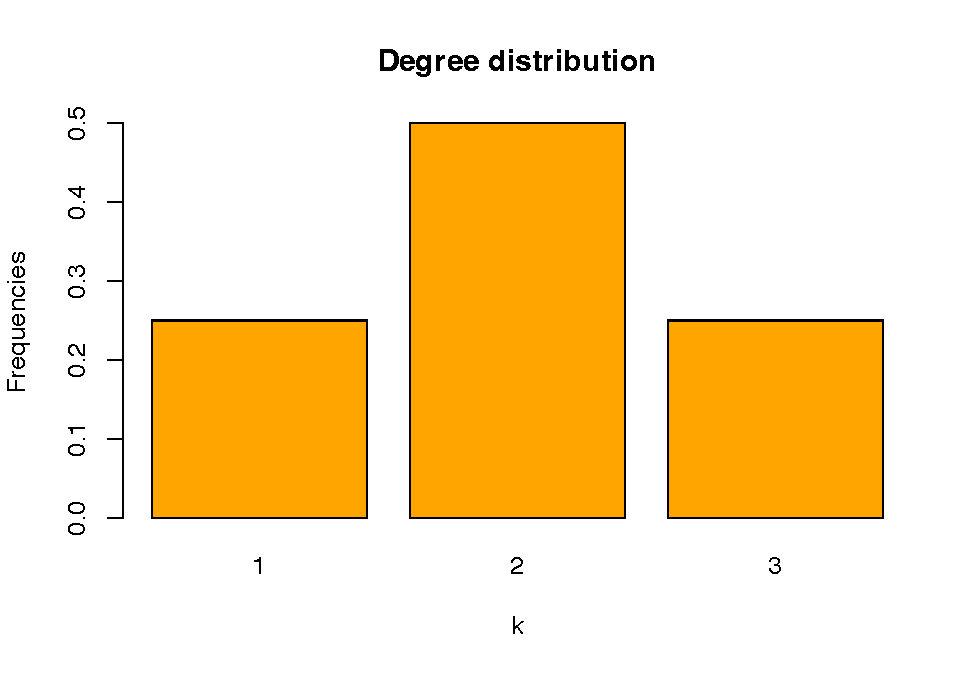
\includegraphics{netsci_files/figure-latex/unnamed-chunk-20-1.pdf}

\hypertarget{adjacency-matrix}{%
\section{Adjacency matrix}\label{adjacency-matrix}}

The adjacency matrix of a network that has \(N\) nodes has \(N\) rows and \(N\) columns. If there is a link from node \(i\) to node \(j\), then \(A_ij = 1\). If node \(i\) and node \(j\) are not connected, then \(A_ij = 0\).

For an undirected network, the link \((i, j)\) has two representations: \(A_ij\) = \(A_ji\). That's why the adjacency matrix of an undirected network is always symmetric.

Lets have a look at the adjacency matrix of \texttt{g1} and \texttt{g2}.

For \texttt{g1}:

\begin{Shaded}
\begin{Highlighting}[]
\FunctionTok{par}\NormalTok{(}\AttributeTok{mar =} \FunctionTok{c}\NormalTok{(}\DecValTok{1}\NormalTok{, }\DecValTok{1}\NormalTok{, }\DecValTok{1}\NormalTok{, }\DecValTok{1}\NormalTok{))}
\FunctionTok{plot}\NormalTok{(g1)}
\end{Highlighting}
\end{Shaded}

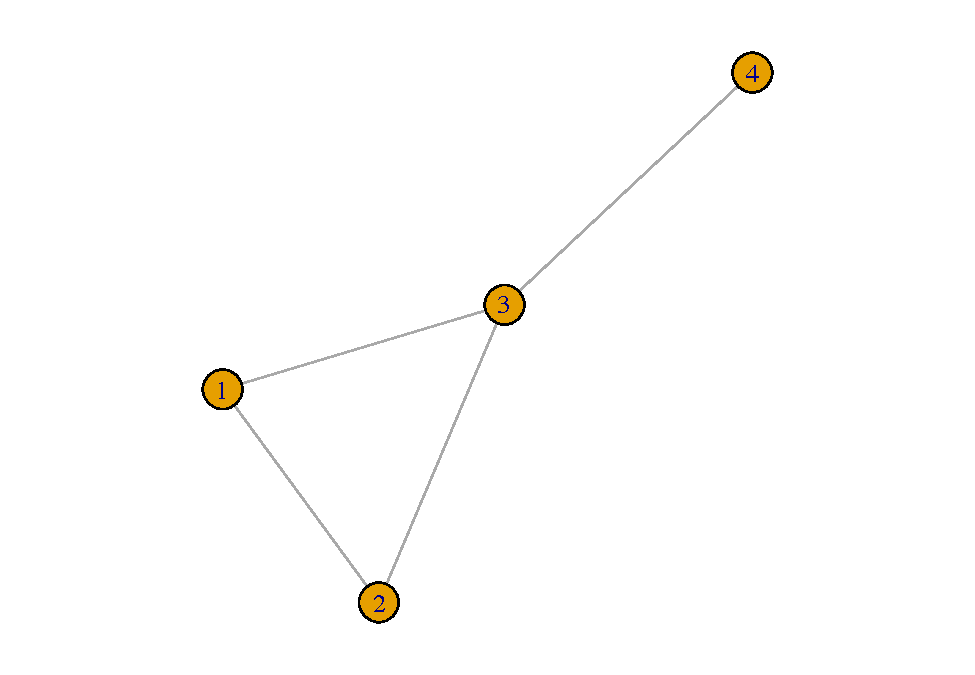
\includegraphics{netsci_files/figure-latex/unnamed-chunk-21-1.pdf}

\begin{Shaded}
\begin{Highlighting}[]
\FunctionTok{as\_adjacency\_matrix}\NormalTok{(g1)}
\end{Highlighting}
\end{Shaded}

\begin{verbatim}
## 4 x 4 sparse Matrix of class "dgCMatrix"
##             
## [1,] . 1 1 .
## [2,] 1 . 1 .
## [3,] 1 1 . 1
## [4,] . . 1 .
\end{verbatim}

For \texttt{g2}:

\begin{Shaded}
\begin{Highlighting}[]
\FunctionTok{par}\NormalTok{(}\AttributeTok{mar =} \FunctionTok{c}\NormalTok{(}\DecValTok{1}\NormalTok{, }\DecValTok{1}\NormalTok{, }\DecValTok{1}\NormalTok{, }\DecValTok{1}\NormalTok{))}
\FunctionTok{plot}\NormalTok{(g2)}
\end{Highlighting}
\end{Shaded}

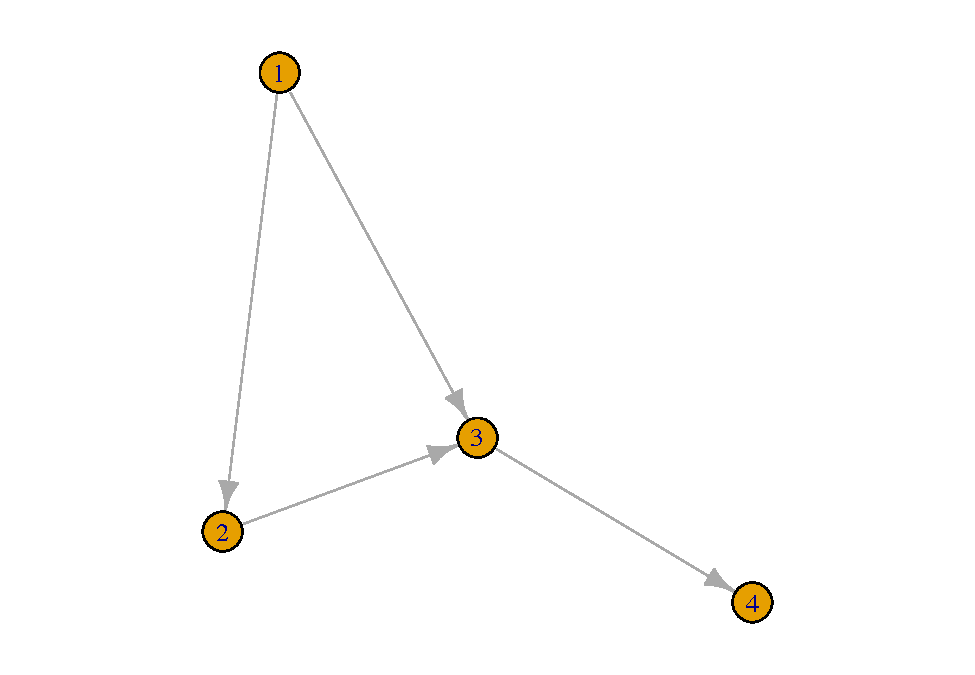
\includegraphics{netsci_files/figure-latex/unnamed-chunk-23-1.pdf}

\begin{Shaded}
\begin{Highlighting}[]
\FunctionTok{as\_adjacency\_matrix}\NormalTok{(g2)}
\end{Highlighting}
\end{Shaded}

\begin{verbatim}
## 4 x 4 sparse Matrix of class "dgCMatrix"
##             
## [1,] . 1 1 .
## [2,] . . 1 .
## [3,] . . . 1
## [4,] . . . .
\end{verbatim}

Each dot in the matrix means \(0\). The adjacency matrices here did not label the column name. To better understand it, you can imagine that the columns are also labeled as {[}1, {]}, {[}2, {]}, {[}3, {]} and {[}4, {]} as the rows are.

\hypertarget{chapter-2-homework}{%
\section{Chapter 2 Homework}\label{chapter-2-homework}}

\begin{rmdnote}
This part is based on Professor YY's module 2 assignment of \href{https://github.com/yy/netsci-course/blob/master/m02-whynetworks/friendship_paradox.ipynb}{measuring the friendship paradox}.
\end{rmdnote}

You can find the homework \href{https://github.com/yy/netsci-course/blob/master/m02-whynetworks/friendship_paradox.ipynb}{here}.

The following task prompts are based on the above homework. You can use them to keep practicing coding in Python.

\hypertarget{task-2-1-networkx-basics}{%
\subsection{\texorpdfstring{Task 2-1: \texttt{Networkx} Basics}{Task 2-1: Networkx Basics}}\label{task-2-1-networkx-basics}}

\begin{itemize}
\item
  2-1-1. Import \texttt{networkx} as \texttt{nx}.
\item
  2-1-2. Set both random seed and numpy random seed to be \texttt{42}.
\item
  2-1-3. Create a networkx graph named \texttt{my\_first\_graph} which contains three nodes and 2 edges, i.e., (1,2) and (2,3).
\item
  2-1-4. In the codes you used for Task \texttt{2-3}: Which element is a \texttt{class}? Which is an \texttt{object}? Which is a \texttt{method}?
\item
  2-1-5. Print the number of nodes in \texttt{my\_first\_graph}. \emph{Hint} : \texttt{len()}
\item
  2-1-6. Print the degree of Node 2, in the format of ``Node 2's degree: m''.
\item
  2-1-7. Print Node 2's neighbors, in the format of ``Node 2's neighbors: {[}m, n, p, q{]}''. \emph{Hint} : \texttt{neighbor()} or \texttt{neighbors()}?

  \begin{itemize}
  \tightlist
  \item
    Note: When you directly return Node 2's neighbors, the result will be \texttt{dict\_keyiterator\ at\ 0x10ec84860}, which is an \href{https://www.w3schools.com/python/python_iterators.asp}{iterator object}. Try to solve this problem either by a for loop or through a \href{https://python-3-patterns-idioms-test.readthedocs.io/en/latest/Comprehensions.html}{list comprehension}
  \end{itemize}
\item
  2-1-8. Print all the node's neighbors in \texttt{my\_first\_graph} in the form of ``Node 1's neighbors: {[}m, n, p, q{]}'' using a python for loop.

  \begin{itemize}
  \tightlist
  \item
    \emph{Hint} : The for loop will iterate over the list returned by the \texttt{nodes()} function.
  \end{itemize}
\item
  2-1-9. Print all the edges in \texttt{my\_first\_graph}.
\item
  2-1-10. Plot \texttt{my\_first\_graph}. \emph{Hint} : \texttt{.draw()}
\end{itemize}

\hypertarget{task-2-2-friendship-paradox-example}{%
\subsection{Task 2-2: Friendship paradox example}\label{task-2-2-friendship-paradox-example}}

\begin{itemize}
\item
  2-2-1. Create a star graph with 20 nodes, and plot it.
\item
  2-2-2. Calculate the average degree of the star graph you just created. Use a for loop to calculate the total degrees.

  \begin{itemize}
  \tightlist
  \item
    \emph{Hint} : You might find the operator of \texttt{+=} useful for \texttt{2-2-2}. \texttt{a\ +=\ b} is short for \texttt{a\ =\ a\ +\ b}.
  \end{itemize}
\item
  2-2-3. Do the same thing using \href{https://numpy.org/doc/stable/reference/generated/numpy.mean.html}{numpy's mean function} which takes in a list and returns the mean of this list.
\end{itemize}

\begin{rmdreminder}
I do not understand Professor YY's note here: ``so if you print a numpy float it will display differently than if you printed a python float, which is why we get the intentional truncation of the value when displayed''.
\end{rmdreminder}

\begin{itemize}
\tightlist
\item
  2-2-4. Get \texttt{star\_graph}'s average degree using networkx's \texttt{info()} function.
\end{itemize}

\hypertarget{task-2-3-generating-random-and-scale-free-networks}{%
\subsection{Task 2-3: Generating random and scale-free networks}\label{task-2-3-generating-random-and-scale-free-networks}}

\begin{itemize}
\item
  2-3-1. Generate a random network with 20 nodes and a connection probability of 0.3. \emph{Hint} : \href{https://networkx.github.io/documentation/stable/reference/generated/networkx.generators.random_graphs.erdos_renyi_graph.html}{\texttt{erdos\_renyi\_graph}}.
\item
  2-3-2. Generate a scale-free network with 20 nodes with each new node having three edges to attach to existing nodes. \emph{Hint} : \href{https://networkx.github.io/documentation/stable/reference/generated/networkx.generators.random_graphs.barabasi_albert_graph.html}{\texttt{barabasi\_albert\_graph()}}
\end{itemize}

\hypertarget{task-2-4-homework-by-professor-yy}{%
\subsection{Task 2-4: Homework by Professor YY}\label{task-2-4-homework-by-professor-yy}}

Answer \href{https://github.com/yy/netsci-course/blob/master/m02-whynetworks/friendship_paradox.ipynb}{Q1 - Q4} as explained by Professor YY.

\hypertarget{SmallWorld}{%
\chapter{Small World Phenomenon}\label{SmallWorld}}

\begin{rmdnote}
The following is not originally from me, but my notes from reading \href{http://networksciencebook.com/}{\emph{Network Science}} (Ch. 2.6-2.10) by \href{https://barabasi.com/}{Albert-László Barabási}. Notes are accompanied by my explanations.
\end{rmdnote}

Before we can understand the small world phenomenon, we need to have more basic knowledge about a network: shortest path, average path length, Breath-first search algorithm, components, and local and average clustering coefficient.

\hypertarget{weight-paths-connectedness-and-clustering}{%
\section{Weight, paths, connectedness, and clustering}\label{weight-paths-connectedness-and-clustering}}

\hypertarget{weighted-network}{%
\subsection{Weighted network}\label{weighted-network}}

So far, we have assumed that the weight of all links in a network is the same. However, networks can be weighted. Take social network as an example. Although you are connected to many people, the weight of these connections is unequal. You probably talk to your family and your close friends more often than to your acquaintances. In an adjacency matrix, suppose you are represented by node \(i\), your mom node \(j\) and one of your acquaintances node \(m\). Also suppose the weight of the link between you and your mom is \(10\), which is ten times the weight of the link between you and the acquaintance. Then we have \(A_{ij} = 10\) and \(A_{im} = 1\).

\hypertarget{shortest-path-network-diameter-and-average-path-length}{%
\subsection{Shortest path, network diameter, and average path length}\label{shortest-path-network-diameter-and-average-path-length}}

\hypertarget{shortest-path}{%
\subsubsection{Shortest path}\label{shortest-path}}

In the real world, objects have physical distances between each other, and that's why we need to fly for three hours from New York to Florida. In networks, physical distances are replaced by \textbf{path lengths}: how many links does the path contain?

For example, in \texttt{g1}, the path length between node \(1\) and node \(4\) can either be 2 (\(1 \to 3 \to 4\)) or 3 (\(1 \to 2 \to 3 \to 4\)):

\begin{Shaded}
\begin{Highlighting}[]
\FunctionTok{par}\NormalTok{(}\AttributeTok{mar =} \FunctionTok{c}\NormalTok{(}\DecValTok{1}\NormalTok{, }\DecValTok{1}\NormalTok{, }\DecValTok{1}\NormalTok{, }\DecValTok{1}\NormalTok{))}
\FunctionTok{plot}\NormalTok{(g1)}
\end{Highlighting}
\end{Shaded}

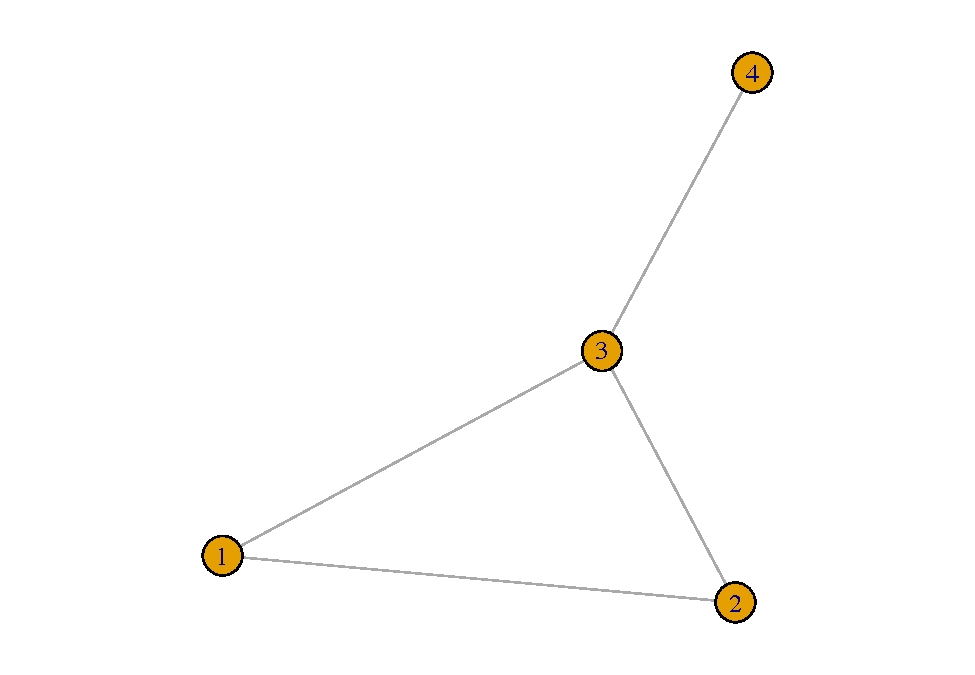
\includegraphics{netsci_files/figure-latex/unnamed-chunk-28-1.pdf}

Obviously, the path length of \(2\) is smaller than \(3\). In this case, \(1 \to 3 \to 4\) is the \textbf{shortest path} (denoted as \(d_{i,j}\)), which is defined as the path with the fewest number of links. In the above example, \(d_{1,4}\) = 2.

In an undirected network, \(d_{i,j} = d_{j,k}\). This often does not hold true in a directed network because:

\begin{enumerate}
\def\labelenumi{\arabic{enumi}.}
\item
  The existence of \((i, j)\) does not guarantee the existence of \((j, i)\);
\item
  Even if both \((i, j)\) and \((j, i)\), the two often are unequal to each other.
\end{enumerate}

For example,

\begin{Shaded}
\begin{Highlighting}[]
\NormalTok{g3 }\OtherTok{\textless{}{-}} \FunctionTok{graph}\NormalTok{( }\AttributeTok{edges=}\FunctionTok{c}\NormalTok{(}\DecValTok{1}\NormalTok{,}\DecValTok{2}\NormalTok{, }\DecValTok{1}\NormalTok{,}\DecValTok{3}\NormalTok{, }\DecValTok{2}\NormalTok{,}\DecValTok{3}\NormalTok{, }\DecValTok{3}\NormalTok{,}\DecValTok{4}\NormalTok{, }\DecValTok{4}\NormalTok{,}\DecValTok{2}\NormalTok{), }\AttributeTok{n=}\DecValTok{4}\NormalTok{, }\AttributeTok{directed=}\ConstantTok{TRUE}\NormalTok{)}
\FunctionTok{par}\NormalTok{(}\AttributeTok{mar =} \FunctionTok{c}\NormalTok{(}\DecValTok{1}\NormalTok{, }\DecValTok{1}\NormalTok{, }\DecValTok{1}\NormalTok{, }\DecValTok{1}\NormalTok{))}
\FunctionTok{plot}\NormalTok{(g3)}
\end{Highlighting}
\end{Shaded}

\begin{figure}

{\centering 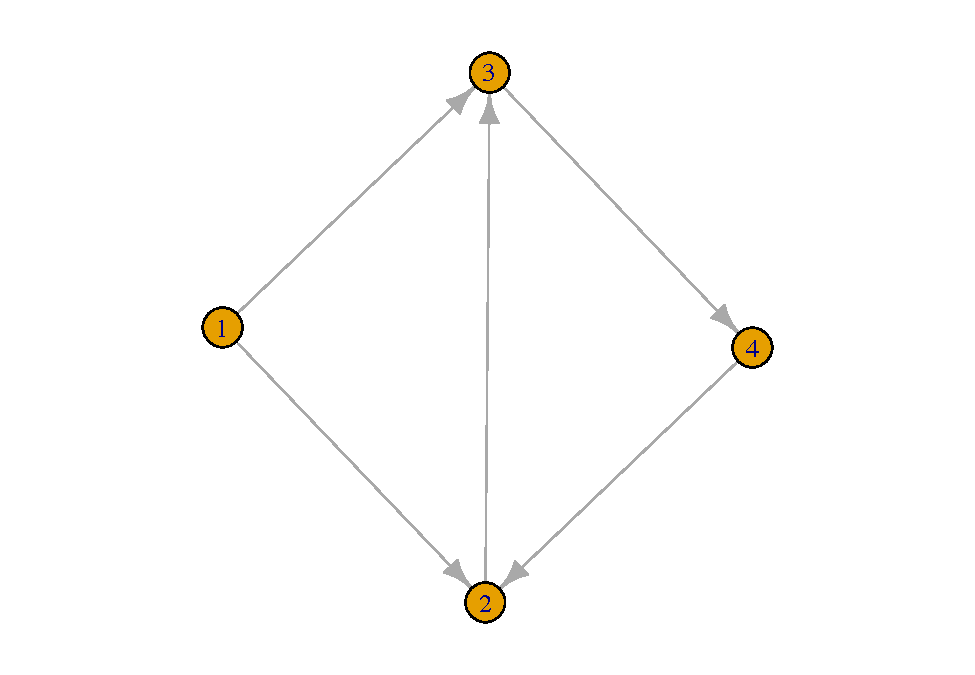
\includegraphics{netsci_files/figure-latex/g3-1} 

}

\caption{shortest paths in a directed network}\label{fig:g3}
\end{figure}

There are paths (\(1 \to 2\), and \(1 \to 3 \to 4 \to 2\)) from node \(1\) to node \(2\) but we don't have on any from node \(2\) to node \(1\). Furthermore, \(d_{2, 4} = 2\) whereas \(d_{4,2} = 1\).

\begin{rmdimportant}
Please note that all the above discussions on shortest path lenghts are based on the assumption that it is a simple contagion. In a complex contagion, things are very different because multiple reinforcements are necessary. Read \citet{centola2007complex} for more detailed explanations.
\end{rmdimportant}

\hypertarget{network-diameter}{%
\subsubsection{Network diameter}\label{network-diameter}}

Among all the shortest paths in a network, the longest one is called the \textbf{diameter} of this network, denoted as \(d_{max}\). In the above Network \ref{fig:g3}, \(d_{max} = 2\): \(d_{1,4} = d_{2,4} = 2\).

\hypertarget{average-path-length}{%
\subsubsection{Average path length}\label{average-path-length}}

Average path length is defined as the average length of shortest paths between any two nodes. For example, in Network \ref{fig:g3}, \(d_{1,2} = d_{1,3} = d_{2,3} = d_{3,4} = d_{4,2} = 1\), \(d_{1,4} = d_{2,4} = d_{3,2} = d_{4,3} = 2\). Therefore, the average is \(\frac{(1 \cdot 5 + 2 \cdot 4)}{5 + 4} = 1.44\). Lets test it:

\begin{Shaded}
\begin{Highlighting}[]
\FunctionTok{average.path.length}\NormalTok{(g3)}
\end{Highlighting}
\end{Shaded}

\begin{verbatim}
## Warning: `average.path.length()` was deprecated in igraph 2.0.0.
## i Please use `mean_distance()` instead.
## This warning is displayed once every 8 hours.
## Call `lifecycle::last_lifecycle_warnings()` to see where this warning was
## generated.
\end{verbatim}

\begin{verbatim}
## [1] 1.444444
\end{verbatim}

\hypertarget{breath-first-search-bfs-algorithm}{%
\subsubsection{Breath-first search (BFS) algorithm}\label{breath-first-search-bfs-algorithm}}

As the size of a network gets larger, it will be more difficult to know what is the shortest path between a pair of nodes. For example, without using computers,

For example, in the network @ref9fig:random3-10 below, what is the shortest path from node \(3\) to node \(90\)?

\begin{Shaded}
\begin{Highlighting}[]
\FunctionTok{set.seed}\NormalTok{(}\DecValTok{42}\NormalTok{)}
\NormalTok{random3 }\OtherTok{\textless{}{-}} \FunctionTok{erdos.renyi.game}\NormalTok{(}\DecValTok{100}\NormalTok{, }\FloatTok{0.1}\NormalTok{, }\AttributeTok{type =} \StringTok{"gnp"}\NormalTok{)}
\end{Highlighting}
\end{Shaded}

\begin{verbatim}
## Warning: `erdos.renyi.game()` was deprecated in igraph 0.8.0.
## i Please use `sample_gnp()` instead.
## This warning is displayed once every 8 hours.
## Call `lifecycle::last_lifecycle_warnings()` to see where this warning was
## generated.
\end{verbatim}

\begin{Shaded}
\begin{Highlighting}[]
\FunctionTok{plot}\NormalTok{(random3)}
\end{Highlighting}
\end{Shaded}

\begin{figure}

{\centering 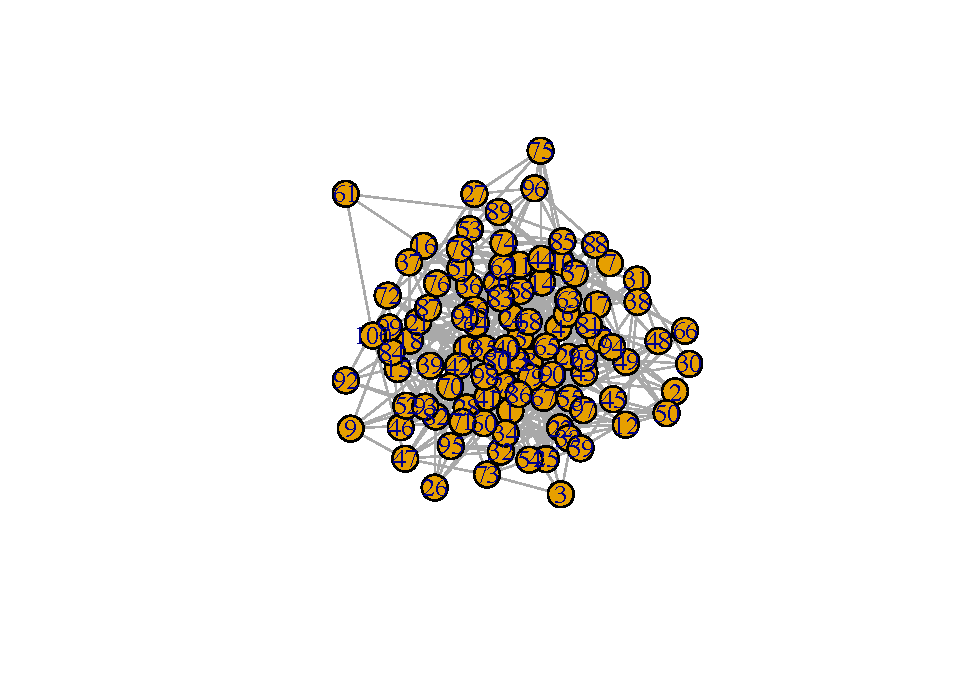
\includegraphics[width=1\linewidth]{netsci_files/figure-latex/random3-1-1} 

}

\caption{A random network to explain Breath-first search (BFS) algorithm}\label{fig:random3-1}
\end{figure}

We are not even sure whether the two nodes are connected or not, let alone knowing the shortest path. Of course, computers can do this very fast:

\begin{Shaded}
\begin{Highlighting}[]
\FunctionTok{shortest\_paths}\NormalTok{(random3, }\AttributeTok{from =} \DecValTok{3}\NormalTok{, }\AttributeTok{to =} \DecValTok{90}\NormalTok{)}
\end{Highlighting}
\end{Shaded}

\begin{verbatim}
## $vpath
## $vpath[[1]]
## + 4/100 vertices, from 071e715:
## [1]  3  8 28 90
## 
## 
## $epath
## NULL
## 
## $predecessors
## NULL
## 
## $inbound_edges
## NULL
\end{verbatim}

From the result, we know that \(d_{3, 90} = 3\). The path is: \(3 \to 8 \to 28 \to 90\). But how did the computer find this path?

The most frequently used algorithm to find the shortest path between two nodes is called ``Breadth-First Search (BFS)''. It starts from the ``source'' node, which is labeled as \(0\). Neighbors of the ``source'' node is then labeled as \(1\), then the neighbors' neighbors, until it reaches the ``target'' node.

For example, we are interested in knowing the shortest path from the source node (``S'') to the target (``T'') in the following Network \ref{fig:bfs01}:

\begin{figure}

{\centering \includegraphics[width=0.55\linewidth]{images/bfs01} 

}

\caption{Illustrating breadth-first search algorithm: source and target}\label{fig:bfs01}
\end{figure}

The breadth-first search algorithm is shown in Figure \ref{fig:bfs} below:

\begin{figure}

{\centering \includegraphics[width=0.5\linewidth]{images/bfs02} \includegraphics[width=0.5\linewidth]{images/bfs03} \includegraphics[width=0.5\linewidth]{images/bfs04} 

}

\caption{Illustrating breadth-first search algorithm: steps}\label{fig:bfs}
\end{figure}

We can see that the shortest path from the ``source'' to the ``target'' is \(3\).

\hypertarget{connectedness}{%
\subsection{Connectedness}\label{connectedness}}

In a disconnected network, subnetworks are called \emph{components} or \emph{clusters}. A \emph{bridge} can connect two components.

For a large network, there are two ways to find out whether it consists of \emph{components}:

\begin{enumerate}
\def\labelenumi{\arabic{enumi}.}
\item
  Using linear algebra to look at the network's adjacency matrix could be rearranged into a block diagonal;
\item
  Using BSF algorithm.
\end{enumerate}

For example, in Figure \ref{fig:disconnected}, the network contains two components:

\begin{Shaded}
\begin{Highlighting}[]
\NormalTok{disconnectedG }\OtherTok{\textless{}{-}} \FunctionTok{graph}\NormalTok{( }\AttributeTok{edges=}\FunctionTok{c}\NormalTok{(}\DecValTok{1}\NormalTok{,}\DecValTok{2}\NormalTok{, }\DecValTok{1}\NormalTok{,}\DecValTok{3}\NormalTok{, }\DecValTok{2}\NormalTok{,}\DecValTok{3}\NormalTok{, }\DecValTok{1}\NormalTok{,}\DecValTok{4}\NormalTok{, }\DecValTok{5}\NormalTok{,}\DecValTok{6}\NormalTok{), }
                        \AttributeTok{n=}\DecValTok{6}\NormalTok{, }
                        \AttributeTok{directed=}\ConstantTok{FALSE}\NormalTok{)}
\FunctionTok{par}\NormalTok{(}\AttributeTok{mar =} \FunctionTok{c}\NormalTok{(}\DecValTok{1}\NormalTok{, }\DecValTok{1}\NormalTok{, }\DecValTok{1}\NormalTok{, }\DecValTok{1}\NormalTok{))}
\FunctionTok{plot}\NormalTok{(disconnectedG)}
\end{Highlighting}
\end{Shaded}

\begin{figure}

{\centering 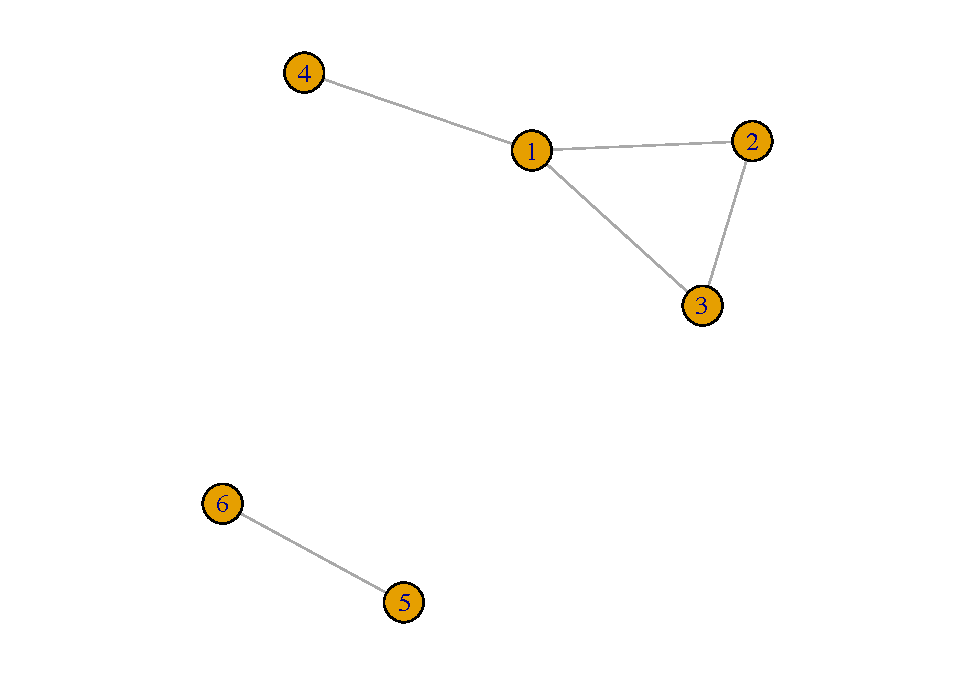
\includegraphics{netsci_files/figure-latex/disconnected-1} 

}

\caption{An example of disconnected network}\label{fig:disconnected}
\end{figure}

In its adjacency matrix, nonzero elements are contained in square blocks along the diagonal and all the remaining elements are zeros:

\begin{figure}

{\centering \includegraphics[width=0.45\linewidth]{images/blockDiagonal} 

}

\caption{Adjacency matrix of the disconnected network}\label{fig:BDmatrix}
\end{figure}

If the components are bridged:

\begin{Shaded}
\begin{Highlighting}[]
\NormalTok{connectedG }\OtherTok{\textless{}{-}} \FunctionTok{graph}\NormalTok{( }\AttributeTok{edges=}\FunctionTok{c}\NormalTok{(}\DecValTok{1}\NormalTok{,}\DecValTok{2}\NormalTok{, }\DecValTok{1}\NormalTok{,}\DecValTok{3}\NormalTok{, }\DecValTok{2}\NormalTok{,}\DecValTok{3}\NormalTok{, }\DecValTok{1}\NormalTok{,}\DecValTok{4}\NormalTok{, }\DecValTok{3}\NormalTok{,}\DecValTok{5}\NormalTok{, }\DecValTok{5}\NormalTok{,}\DecValTok{6}\NormalTok{), }\AttributeTok{n=}\DecValTok{6}\NormalTok{, }
                     \AttributeTok{directed=}\ConstantTok{FALSE}\NormalTok{)}
\FunctionTok{par}\NormalTok{(}\AttributeTok{mar =} \FunctionTok{c}\NormalTok{(}\DecValTok{1}\NormalTok{, }\DecValTok{1}\NormalTok{, }\DecValTok{1}\NormalTok{, }\DecValTok{1}\NormalTok{))}
\FunctionTok{plot}\NormalTok{(connectedG)}
\end{Highlighting}
\end{Shaded}

\begin{figure}

{\centering 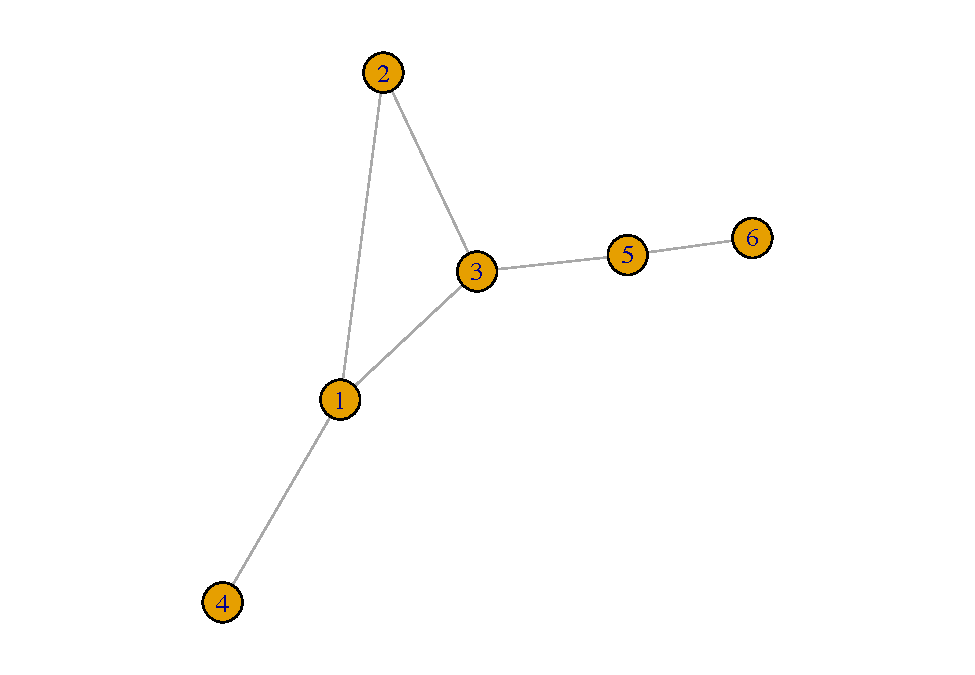
\includegraphics{netsci_files/figure-latex/blockDiagonal02-1} 

}

\caption{An example of connected network}\label{fig:blockDiagonal02}
\end{figure}

Then its adjacency matrix cannot be rearranged in a block diagonal form:

\begin{verbatim}
## 6 x 6 sparse Matrix of class "dgCMatrix"
##                 
## [1,] . 1 1 1 . .
## [2,] 1 . 1 . . .
## [3,] 1 1 . . 1 .
## [4,] 1 . . . . .
## [5,] . . 1 . . 1
## [6,] . . . . 1 .
\end{verbatim}

Then how can we find whether a network is connected or disconnected using BFS algorithm?

It's very easy. In a connected network, we can reach all the nodes from the ``source node''. Therefore, the number of labeled nodes is equal to the size of the network, \(N\). However, in a disconnected network, nodes in different components cannot be reached, so the number of labeled nodes is smaller than \(N\).

To illustrate, let's go back to the network \ref{fig:bfs01}. This time, we add a component consisting two nodes to it.

\begin{figure}

{\centering \includegraphics[width=0.65\linewidth]{images/bfsD1} 

}

\caption{A disconnected network composed of two components}\label{fig:bfsD1}
\end{figure}

We apply BFS algorithm to the network \ref{fig:bfsD1}. The starting point is the same as above. You can see that the process ceased when the label reaches \(3\):

\begin{figure}

{\centering \includegraphics[width=0.65\linewidth]{images/bfsD2} 

}

\caption{BFS stops in a disconnected network}\label{fig:bfsD2}
\end{figure}

How can we identify the remaining component(s)? In the example above, we assign label \(4\) to a randomly unlabeled node \(j\) and all the other nodes reachable from node \(j\).

\begin{figure}

{\centering \includegraphics[width=0.65\linewidth]{images/bfsD3} 

}

\caption{Identifying components in a disconnected network through BFS algorithm}\label{fig:bfsD3}
\end{figure}

What if there are multiple components? It's the same as the above step. After labeling all reachable nodes, if the number of labeled nodes is still smaller than \(N\), then we assign label \(5\) to a randomly unlabeled node \(m\), and all other nodes reachable from node \(m\). The process goes on until the number of labeled nodes is equal to \(N\).

\hypertarget{clustering-coefficient}{%
\subsection{Clustering coefficient}\label{clustering-coefficient}}

To what degree are a node's neighbors connected with each other? That's what clustering coefficient measures.

If the degree of node \(i\) is \(k_i\), then node \(i\)'s \textbf{local clustering coefficient} is defined as

\begin{equation}
\begin{split}
  C_i & = L_i ÷ \frac{k_i \cdot (k_i - 1)}{2} \\
  & = \frac{2 \cdot L_i}{k_i \cdot (k_i - 1)}
\end{split}
\label{eq:localClustering}
\end{equation}

\(L_i\) represents the actual number of links between node \(i\)'s \(k_i\) neighbors, and \(\frac{k_i \cdot (k_i - 1)}{2}\) means the highest number of links possible between those neighbors.

\textbf{Local clustering coefficient} of a node is the probability that two neighbors of a given node has a link to each other. It measures the local density of links in a network.

\textbf{Local clustering coefficient} is for nodes. If we are interested in the degree of clustering for a network, we need to calculate \textbf{average clustering coefficient}, denoted as \(\langle C \rangle\) which is simply the average of local clustering coefficient of all the nodes in a given network:

\begin{equation}
   \langle C \rangle = \frac{1}{N} \cdot \sum_{i = 1}^N C_i
\label{eq:avergeClustering}
\end{equation}

\hypertarget{chapter-3-homework}{%
\section{Chapter 3 Homework}\label{chapter-3-homework}}

\begin{rmdnote}
This part is based on Professor YY's module 3 assignment of \href{https://github.com/yy/netsci-course/blob/master/m03-smallworld/shortest_path_length_distribution.ipynb}{shortest path length distribution}.
\end{rmdnote}

You can find the homework \href{https://github.com/yy/netsci-course/blob/master/m03-smallworld/shortest_path_length_distribution.ipynb}{here}.

\hypertarget{weak-ties-and-watts-strogatz-model}{%
\chapter{Weak Ties and Watts-Strogatz model}\label{weak-ties-and-watts-strogatz-model}}

In this chapter, we are going to learn how to generate random networks. Then, we will study some important characteristics of random networks, such as average degree, and degree distribution. We are also going to read two of the most influential papers and get an idea of weak ties and Watts-Strogatz model.

\hypertarget{random-networks-barabuxe1si-ch.3}{%
\section{Random networks (Barabási Ch.3)}\label{random-networks-barabuxe1si-ch.3}}

\begin{rmdnote}
The following is not originally from me, but my notes from reading \href{http://networksciencebook.com/}{\emph{Network Science}} (Ch. 3) by \href{https://barabasi.com/}{Albert-László Barabási}. Notes are accompanied by my explanations.
\end{rmdnote}

\hypertarget{generating-a-random-network}{%
\subsection{Generating a random network}\label{generating-a-random-network}}

Most of networks in real life look like randomly constructed. Then, how can we, as humans, produce random networks that we see in nature?

Simply by putting links randomly between nodes.

But how can we make sure that we are putting links \textbf{randomly}?

Think about it for a minute before reading on.

If you have studied statistics, you would know that \textbf{randomness} is all about \textbf{probability}. If we say that we are going to \textbf{randomly} pick a person from a group, then we'll need to make sure that \textbf{each} person in the group has an \textbf{equal} chance to be picked. Otherwise, the choice is not \textbf{random}.

Now, let's go back to our original problem: how can we \textbf{randomly} put links between nodes?

For example, we now have 100 isolated nodes, which are called \textbf{singletons}, as shown below. What to do next?

\begin{Shaded}
\begin{Highlighting}[]
\NormalTok{g4\_1 }\OtherTok{\textless{}{-}} \FunctionTok{graph}\NormalTok{( }\AttributeTok{edges=}\ConstantTok{NULL}\NormalTok{, }\AttributeTok{n=}\DecValTok{100}\NormalTok{)}
\FunctionTok{plot}\NormalTok{(g4\_1)}
\end{Highlighting}
\end{Shaded}

\begin{figure}

{\centering 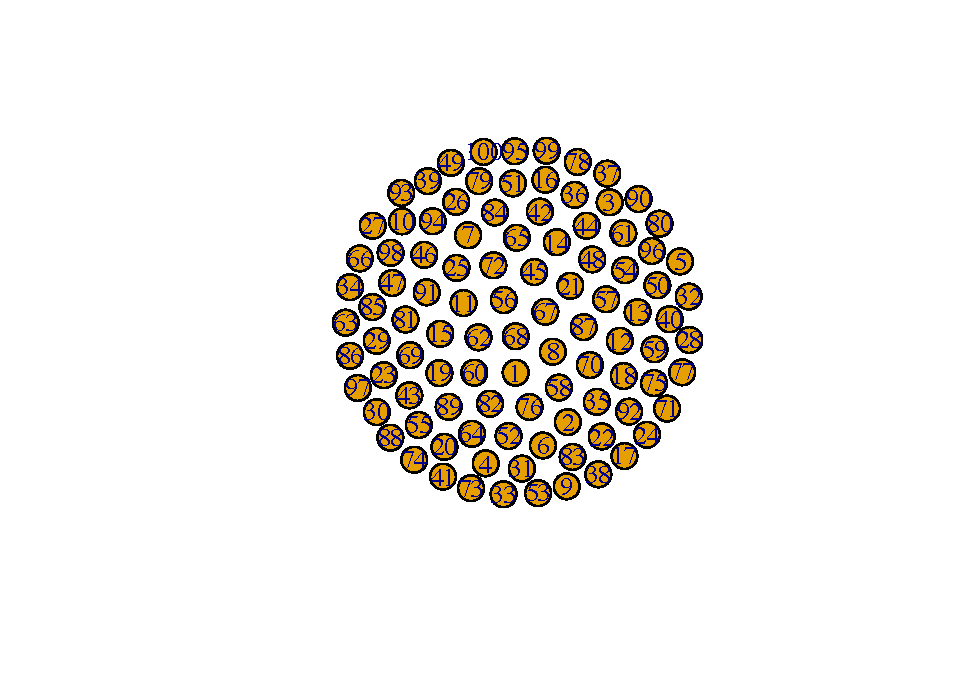
\includegraphics[width=1\linewidth]{netsci_files/figure-latex/g4-1-1} 

}

\caption{100 isolated nodes}\label{fig:g4-1}
\end{figure}

Frist, we'll set up a value \emph{p} (\(0 \leq p \leq 1\)), called \textbf{link probability}. Then, we'll pick a pair of nodes (STEP 1), for example, \(i\) and \(j\), and generate a ramdom number \(r\) for this pair (STEP 2). If \(r < p\), then we connect \(i\) and \(j\). Otherwise, we keep them disconnected. We'll repeat step 1 and step 2 for all node pairs, the total number of which should be \(\frac{N(N-1)}{2}\). This way, we will make sure that the probability of each pair being connected is exactly \(p\). Why so?

\begin{Shaded}
\begin{Highlighting}[]
\FunctionTok{plot}\NormalTok{(}\FunctionTok{c}\NormalTok{(}\DecValTok{0}\NormalTok{, }\DecValTok{1}\NormalTok{), }\FunctionTok{c}\NormalTok{(}\DecValTok{0}\NormalTok{, }\FloatTok{0.2}\NormalTok{), }
     \AttributeTok{type=} \StringTok{"n"}\NormalTok{, }
     \AttributeTok{xlab =} \StringTok{""}\NormalTok{, }
     \AttributeTok{ylab =} \StringTok{""}\NormalTok{, }
     \AttributeTok{yaxt=}\StringTok{"none"}\NormalTok{)}
\CommentTok{\# Solution: https://rstudio{-}pubs{-}static.s3.amazonaws.com/}
\CommentTok{\# 297778\_5fce298898d64c81a4127cf811a9d486.html}
\FunctionTok{abline}\NormalTok{(}\AttributeTok{v=}\FloatTok{0.1}\NormalTok{, }\AttributeTok{col=}\StringTok{"red"}\NormalTok{)}
\FunctionTok{rect}\NormalTok{(}\DecValTok{0}\NormalTok{,}\DecValTok{0}\NormalTok{,}\FloatTok{0.1}\NormalTok{,}\FloatTok{0.2}\NormalTok{,}\AttributeTok{col=}\StringTok{"lightgreen"}\NormalTok{)}
\FunctionTok{rect}\NormalTok{(}\FloatTok{0.1}\NormalTok{,}\DecValTok{0}\NormalTok{,}\DecValTok{1}\NormalTok{,}\FloatTok{0.2}\NormalTok{,}\AttributeTok{col=}\StringTok{"red"}\NormalTok{)}
\end{Highlighting}
\end{Shaded}

\begin{figure}

{\centering 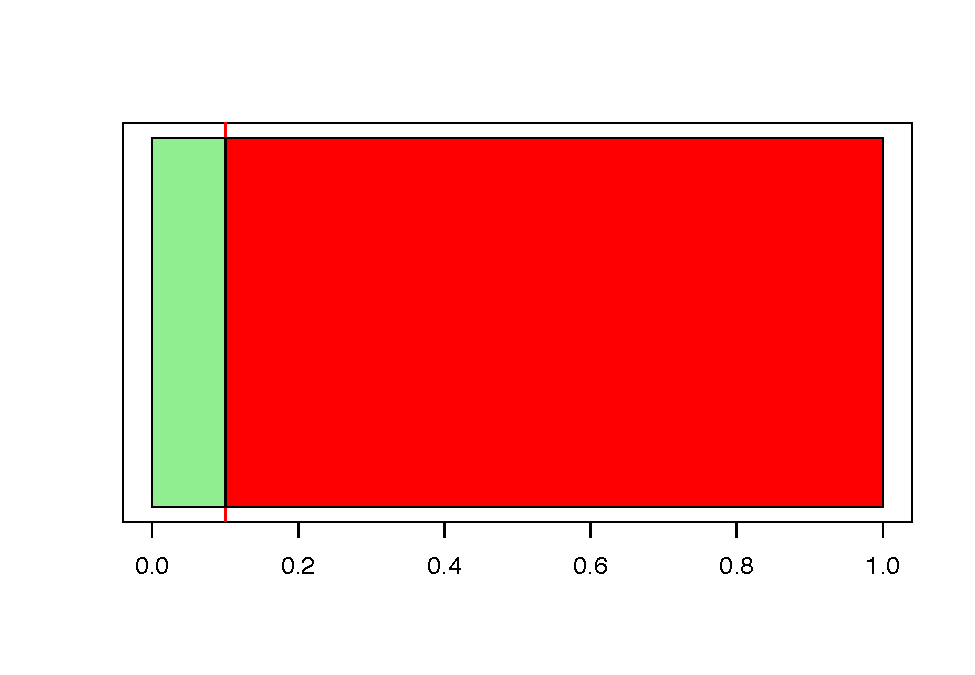
\includegraphics{netsci_files/figure-latex/1-9-1} 

}

\caption{Illustrating why the probability of each pair being connected is equal to the link probability}\label{fig:1-9}
\end{figure}

The reason can be shown in Figure \ref{fig:1-9}. If we set \(p = 0.1\), then only \(10\%\) of random numbers will fall in the range of \([0,0.1)\) (the area shown in light green), the remaining \(90\%\) will fall in \([0.1,1]\)\footnote{I am a little bit uncertain here because I don't know where to put 0.1.}.

Okay, let's set \(p=0.1\) and see what will happen:

\begin{Shaded}
\begin{Highlighting}[]
\CommentTok{\# Solution from: https://rpubs.com/lgadar/generate{-}graphs}
\FunctionTok{set.seed}\NormalTok{(}\DecValTok{42}\NormalTok{)}
\NormalTok{erdosRenyi }\OtherTok{\textless{}{-}} \FunctionTok{erdos.renyi.game}\NormalTok{(}\DecValTok{100}\NormalTok{, }\FloatTok{0.1}\NormalTok{, }\AttributeTok{type =} \StringTok{"gnp"}\NormalTok{)}
\FunctionTok{plot}\NormalTok{(erdosRenyi)}
\end{Highlighting}
\end{Shaded}

\begin{figure}

{\centering 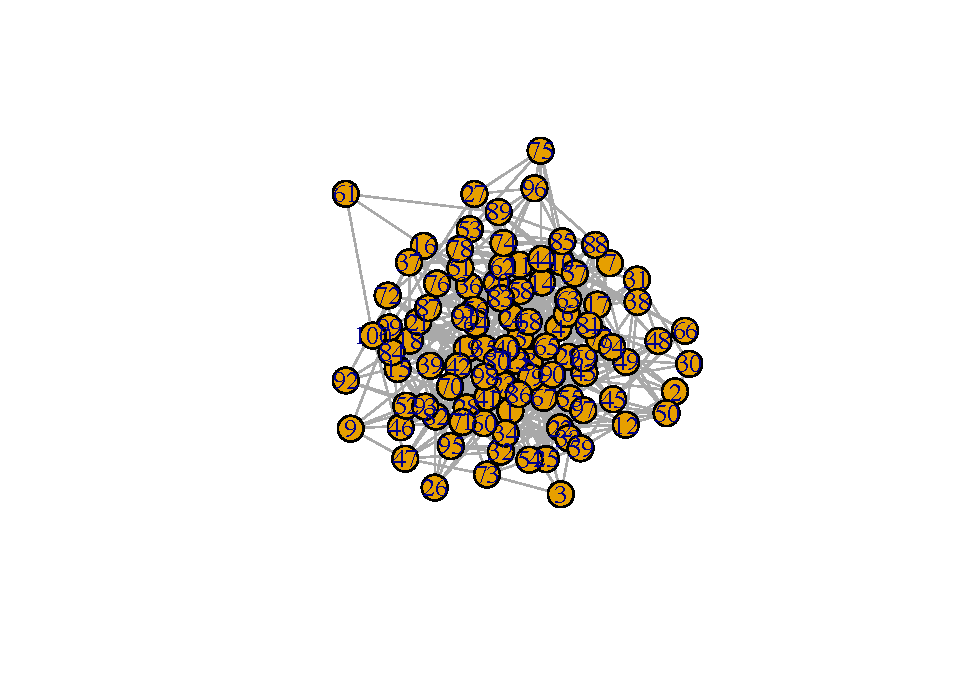
\includegraphics[width=1\linewidth]{netsci_files/figure-latex/erdosRenyi-1} 

}

\caption{An Erdős-Rényi network}\label{fig:erdosRenyi}
\end{figure}

The method described above is used in a model called \textbf{\(G(N,p)\) model}, which was introduced independently by Edgar Nelson Gilbert. In this model, the number of nodes (\(N\)), and link probability (\(p\)) are fixed.

There is a similar model called \textbf{\(G(N,L)\) model} where the number of nodes and the number of links are fixed. This model was introduced by Pál Erdős and Alfréd Rényi.

In practice, we use \textbf{\(G(N,p)\) model} more. But since Pál Erdős and Alfréd Rényi played such an important rold in advancing our understanding of random networks, we still name networks generated by the \textbf{\(G(N,p)\) model} as an \textbf{Erdős-Rényi network}.

\begin{rmdcaution}
In \href{http://networksciencebook.com/chapter/3\#random-network}{Chapter 3.2} of \href{http://networksciencebook.com/}{\emph{Network Science}} , there is a mistake: the second step of generating a random network said that ``if the number exceeds \(p\), connect the selected node pair with a link''. However, it should be ``if the number is smaller than p, connect the selected node pair with a link.''
\end{rmdcaution}

\hypertarget{average-degree-and-the-expected-number-of-links-in-a-random-network}{%
\subsection{Average degree, and the expected number of links in a random network}\label{average-degree-and-the-expected-number-of-links-in-a-random-network}}

We can think of the process (of first generating a random number for a pair of nodes, then comparing it with \(p\), and finally deciding whether to link the pair or not) as tossing a coin \citep{menczer2020first}.

Imagine we have a biased coin which gives us heads with probability \(p\), which is equal to the \textbf{link probability} we talked about before. Take \(p=0.1\) as an example. If we toss the coin for ten times, then we are expecting \(10*0.1=1\) head, right? For the same token, when we have \(100\) tosses, we will be expecting \(10\) heads.

In the procudure of random network generation discussed above, we concluded that a pair of nodes being connected has a probability of \(p\), which is the same as the probability of us having a head when we toss a coin. Since we are expecting \(10\) heads out of \(100\) tosses, then how many connected pairs of nodes are expected, or, how many links are expected, if we examine \(100\) pairs? \(10\), right?

How do we get this number? We simply multiply the total number of tosses in the case of flipping coins (or the total number of pairs of nodes we have in the case of random network generation) by \(p\).
Now, in the \(G(N,p)\) model, we have \(N\) nodes. It's easy to understand that we will have \({N \choose 2} = \frac{N(N-1)}{2}\) pairs of nodes to examine. So, \textbf{the number of links we are expecting in this random network} is:

\begin{equation}
  \langle L \rangle = \frac{N(N-1)}{2}p \label{eq:average-L}
\end{equation}

\(\langle L \rangle\) here stands for the \textbf{expected value}. A given random network generated by \(G(N,p)\) does not necessarily have exactly \(\frac{N(N-1)}{2}p\) links. But as we generate more and more random networks using the \(G(N,p)\) model, the average number of links will be \(\frac{N(N-1)}{2}p\). That's what we mean by \textbf{expected value}. You can look at \textbf{Image 3.3} in \href{http://networksciencebook.com/}{\emph{Network Science}} for examples and illustrations.

Then, in this random network, what is the \textbf{average degree}?

Recall Eq. \eqref{eq:AverageDegree}. Replacing \(L\) with \(\langle L \rangle\) from Eq. \eqref{eq:average-L}, we have:

\begin{equation}
  \langle k \rangle = \frac{2\langle L \rangle}{N} = p(N-1) \label{eq:average-D}
\end{equation}

\begin{rmdtip}
How to remember Eq. \eqref{eq:average-D}:

The average degree of a random network is the product of \(p\), the \textbf{link probability}, and \((N-1)\), the maximum number of links (or neighbors) a node can have.
\end{rmdtip}

You can read \href{http://networksciencebook.com/chapter/3\#number-of-links}{Ch. 3.3} of \href{http://networksciencebook.com/}{\emph{Network Science}} for more detailed mathematical reasoning.

\hypertarget{degree-distribution-1}{%
\subsection{Degree distribution}\label{degree-distribution-1}}

\hypertarget{binomial-distribution}{%
\subsubsection{Binomial distribution}\label{binomial-distribution}}

First of all, if you are not familiar with combinations and permutations, or that you have forgotten what you learnt in your high school, you are encouraged to go through \href{https://www.mathsisfun.com/combinatorics/combinations-permutations.html}{this amazing tutorial} on \href{https://www.mathsisfun.com/}{mathsisfun.com}.

Then, carefully read throught \href{https://www.mathsisfun.com/data/binomial-distribution.html}{this tutorial on binomial distribution}.

If you are able to understand the tutorials above, then you should know that if we have a biased coin which produces heads with probability \(p\), the probability of having \(k\) heads out of \(n\) tosses is:

\begin{equation}
  {n \choose k}p^k(1-p)^{n-k} \label{eq:coin-tossing-binomial}
\end{equation}

How to understand it?

We can look at it this way: tossing a coin \(n\) times, we have \(2^n\) different outcomes (i.e., combinations of heads and tails), and the number of outcomes (or combinations, if you want) that have \(k\) heads is \(n\choose k\) outcomes. However, we cannot simply use \({n\choose k}\div{2^n}\) to calculate the probability of having \(k\) heads. Why? Because this is a \textbf{biased} coin, so each outcome (or combination) has different probabilities.

What should we do then?

Now we know the number of outcomes that will produce \(k\) heads out of \(n\) tosses. It will be great if we know the probability of each of these outcomes and sum them up. Bingo!

When we think more deeply, we will know that each of these \(n\choose k\) outcomes has exactly the same probability: \(p^k(1-p)^{n-k}\). But why? Read \href{https://www.mathsisfun.com/data/binomial-distribution.html}{this tutorial on binomial distribution} again, especially the tree diagram. Also, you'll find \href{https://www.mathsisfun.com/data/probability-events-independent.html}{this tutorial} on the probability of independent events helpful.

Now, let's go back to random networks.

\begin{longtable}[]{@{}
  >{\raggedright\arraybackslash}p{(\columnwidth - 6\tabcolsep) * \real{0.2308}}
  >{\raggedright\arraybackslash}p{(\columnwidth - 6\tabcolsep) * \real{0.3590}}
  >{\raggedright\arraybackslash}p{(\columnwidth - 6\tabcolsep) * \real{0.1538}}
  >{\raggedright\arraybackslash}p{(\columnwidth - 6\tabcolsep) * \real{0.2564}}@{}}
\caption{\label{tab:network-and-coin} Comparing random network generation and flipping coins}\tabularnewline
\toprule\noalign{}
\begin{minipage}[b]{\linewidth}\raggedright
\end{minipage} & \begin{minipage}[b]{\linewidth}\raggedright
\(p\)
\end{minipage} & \begin{minipage}[b]{\linewidth}\raggedright
\(N\)
\end{minipage} & \begin{minipage}[b]{\linewidth}\raggedright
\(k\)
\end{minipage} \\
\midrule\noalign{}
\endfirsthead
\toprule\noalign{}
\begin{minipage}[b]{\linewidth}\raggedright
\end{minipage} & \begin{minipage}[b]{\linewidth}\raggedright
\(p\)
\end{minipage} & \begin{minipage}[b]{\linewidth}\raggedright
\(N\)
\end{minipage} & \begin{minipage}[b]{\linewidth}\raggedright
\(k\)
\end{minipage} \\
\midrule\noalign{}
\endhead
\bottomrule\noalign{}
\endlastfoot
random network generation & link probability & number of nodes & number of node pairs successfully connected \\
tossing coins & probability of having a head in one toss & number of tosses & number of heads \\
\end{longtable}

For a given node \(i\), the maximum number of links it can have is \(N-1\). Let's denote the probability of node \(i\) having \(k\) links as \(p^k\). Eq. \eqref{eq:coin-tossing-binomial}, we know that:

\begin{equation}
  p^k = {N-1 \choose k}p^k(1-p)^{N-1-k} \label{eq:random-network-binomial}
\end{equation}

In this binomial distribution, the mean is:

\begin{equation}
  E(x) = Np \label{eq:binomial-mean}
\end{equation}

Its standard deviation is:

\begin{equation}
  \sigma_i = [p(1-p)N]^\frac{1}{2} \label{eq:binomial-sd}
\end{equation}

And its second moment is:

\begin{equation}
  E(x^2) = p(1-p)N + p^2N^2 \label{eq:binomial-2nd-moment}
\end{equation}

Sorry that I am currently not capable of proving Eq. \eqref{eq:binomial-mean} to Eq. \eqref{eq:binomial-2nd-moment}. For now, just memorize them.

\hypertarget{poisson-distribution}{%
\subsubsection{Poisson distribution}\label{poisson-distribution}}

Most real networks are sparce, so its average degree \(\langle k \rangle\) is much smaller than the size of the network, \(N\). Considering this limit, we usually use Poisson distribution to describe a random network's degree distribution because of simplicity:

\begin{equation}
  p_k = e^{-\langle k \rangle}\frac{\langle k \rangle^k}{k!} \label{eq:poisson}
\end{equation}

Eq. \eqref{eq:random-network-binomial} and Eq. \eqref{eq:poisson} are collectively called \textbf{degree dostribution of a random network}.

Things to keep in mind:

\begin{enumerate}
\def\labelenumi{\arabic{enumi}.}
\item
  Binomial form is the exact version; Poisson distribution is only an approximation;
\item
  We'd better use Binomial distribution to describe a small network, for example, \(N = 10^2\), but use Poisson distribution for large networks, for example, \(N = 10^3\) or \(10^4\);
\item
  In Poisson distribution, the standard deviation is \(\sqrt {\langle k \rangle}\);
\item
  The Poisson distribution tells us that for two networks, as long as they have the same \(\langle k \rangle\), their degree distribution is almost exactly the same despite different sizes, i.e., \(N\).
\end{enumerate}

\begin{rmdreminder}
I did not quite understand the lecture on the Poisson distribution by Professor YY.\\
\end{rmdreminder}

\hypertarget{poisson-distribution-does-not-capture-reality}{%
\subsection{Poisson distribution does not capture reality}\label{poisson-distribution-does-not-capture-reality}}

Poisson distribution undoutedly accurately describes the degree distribution of random networks, but we need to ask, do random netwoks reflect reality?

Reading \href{http://networksciencebook.com/chapter/3\#not-poisson}{Ch. 3.5}, will let us know that if random networks can describe social networks in our daily lives, we would expect that:

\begin{enumerate}
\def\labelenumi{\arabic{enumi}.}
\item
  Most people will have \(\langle k \rangle \pm \sqrt {\langle k \rangle}\) friends;
\item
  The highest number of friends a person can have is not that different than the smallest possible number.
\end{enumerate}

However, we know that this is not the case in real life. Many people have over 5,000 contacts on Facebook and WeChat.

From the figure shown in \href{http://networksciencebook.com/chapter/3\#not-poisson}{Ch. 3.5}, we will know that in real networks, both \textbf{the number of high degree nodes}, and \textbf{the standard deviation of the distribution}, are much larger than what is expected from random networks.

\hypertarget{reading-two-seminal-papers}{%
\section{Reading two seminal papers}\label{reading-two-seminal-papers}}

\hypertarget{the-strength-of-weak-ties-by-granovetter1973strength}{%
\subsection{\texorpdfstring{\emph{The Strength of Weak Ties} by \citet{granovetter1973strength}}{The Strength of Weak Ties by @granovetter1973strength}}\label{the-strength-of-weak-ties-by-granovetter1973strength}}

Please read the following articles carefully by yourself before reading my notes.

Granovetter, M. S. (1973). \href{https://www.cs.cmu.edu/~jure/pub/papers/granovetter73ties.pdf}{The strength of weak ties}. \emph{American journal of sociology, 78}(6), 1360-1380.

This is a highly influential paper: more than 58K as of Nov.~2020.

\begin{itemize}
\item
  Overlap in friendship circles: Suppose there are two individuals, \emph{A} \& \emph{B}, and a group of people, \emph{S} = \emph{C}, \emph{D}, \emph{E}. The stronger the tie between \emph{A} and \emph{B}, the more people in Group S will be tied to \textbf{both} A and B.
\item
  If there is a strong tie between \(A\) and \(B\), and between \(A\) and \(C\). It's very likely that \(B\) and \(C\) also are friends, because

  \begin{enumerate}
  \def\labelenumi{\arabic{enumi}.}
  \tightlist
  \item
    A common contact will bring \(B\) and \(C\) into interaction;
  \item
    The stronger the tie, the more similar are individuals to each other. \(A\) is similar to \(B\), and \(A\) is similar to \(C\), and thus \(B\) is similar to \(C\), making it more likely for them to be friends; and
  \item
    If \(B\) and \(C\) are aware of each other but are not friends, they might have a ``psychological strain'' since their feelings are not consistent with \(A\).
  \end{enumerate}
\end{itemize}

Therefore, this tried in Figure \ref{fig:tried} is very unlikely to occur:

\begin{figure}

{\centering \includegraphics[width=0.45\linewidth]{images/tried} 

}

\caption{An impossible tried, adapted from Fig.1 of Granovetter (1973)}\label{fig:tried}
\end{figure}

\begin{itemize}
\item
  A bridge is a link connecting two otherwise disconnected groups. ``No strong tie is a bridge''. All bridges are weak ties.
\item
  A local bridge of \(n\): if this bridge does not exist, what is the shortest path between these two points?
\item
  No strong tie is a local bridge.
\item
  Whatever is is to be diffused can reach a larger number of people if passed through weak rather than strong ties\footnote{\citet{centola2007complex} advanced this idea by distinguishing between complex contagions and simple contagions like an epidemic. They argued that the strength of weak ties should not be simply generalized to complex contagions, which require affirmation from multiple sources. Therefore, not only the length, but also, and maybe more importantly, the width of the ties influences complex contagions.}.
\item
  People are more likely to find jobs through weak ties rather than strong.
\end{itemize}

\begin{rmdreminder}
Something I do not understand yet in this paper:
``Thus, network fragmentation, by reducing drastically the number of paths from any leader to his potential followers, would inhibit trust in such leaders.''
\end{rmdreminder}

\hypertarget{watts-strogatz-model-of-small-world}{%
\subsection{Watts-Strogatz model of small world}\label{watts-strogatz-model-of-small-world}}

Please read the following paper:

Watts, D. J., \& Strogatz, S. H. (1998). \href{http://materias.df.uba.ar/dnla2019c1/files/2019/03/watts-collective_dynamics-nature_1998.pdf}{Collective dynamics of 'small-world'networks}. \emph{Nature, 393}(6684), 440-442.

It's another canonical study in the field of network science, also highly influential.

\href{https://dwulff.github.io/_Networks/Downloads/watts_strogatz.html}{Here} is an amazing tutorial \& practice to understand WS model. And \href{http://worrydream.com/ScientificCommunicationAsSequentialArt/}{here} is another one I found.

\hypertarget{scale-free}{%
\chapter{Scale-Free Networks}\label{scale-free}}

Networks in real life are rarely random. Most of them are ``scale-free''. What does ``scale-free'' mean? What are the defining features of scale-free networks? And how do we generate these networks? These are the topics we are going to cover in this Chapter 5.

\hypertarget{power-law-distributions}{%
\section{Power-Law Distributions}\label{power-law-distributions}}

\begin{rmdnote}
The following came from the online course of \href{https://github.com/yy/netsci-course}{INFO I606} at Indiana University by Professor \href{https://yongyeol.com/}{Yong-Yoel (``YY'') Ahn}.
\end{rmdnote}

\hypertarget{differences-between-fb-study-and-the-milgram-study}{%
\subsection{Differences between FB study and the Milgram study}\label{differences-between-fb-study-and-the-milgram-study}}

The differences between the \href{https://research.fb.com/blog/2016/02/three-and-a-half-degrees-of-separation/}{Facebook study} and the Milgram study:

\begin{enumerate}
\def\labelenumi{\arabic{enumi}.}
\item
  In FB study, researchers knew the whole graph. They would have this in mind when calculating the shortest paths. However, participants in the Milgram study did not know the whole graph;
\item
  There wasn't any lost ``packages'' in FB study.
\end{enumerate}

One thing we need to be cautious with the FB study is that there were quite a number of people having 500-5,000friends, as can be seen in the \href{https://arxiv.org/pdf/1111.4503.pdf}{study PDF}. But is it possible in real life? \href{https://www.newyorker.com/science/maria-konnikova/social-media-affect-math-dunbar-number-friendships}{Dunbar's number} suggests that we as humans can maintain at most 150 friends. Therefore, the FB study might have overestimated the distance between people.

\hypertarget{power-law}{%
\subsection{Power law}\label{power-law}}

\begin{rmdreminder}
Before discussing power-law distributions, Professor YY talked about the connection between binomial, Poisson, and normal distributions. It is beyond my scope of knowledge. However, you are encouraged to read \href{http://www.johndcook.com/blog/normal_approx_to_poisson/}{this} article on this topic.
\end{rmdreminder}

The above picture of the bird came from \href{http://gdut_yy.gitee.io/doc-csstdg4/ch8.html\#_8-2-padding}{here}.

Check out \href{https://www.youtube.com/watch?v=fCn8zs912OE}{this video} to understand \textbf{Zipf's law}. Also, \href{https://www.hpl.hp.com/research/idl/papers/ranking/ranking.html}{here} is an amazing tutorial\footnote{I haven't throughly read and understood it yet\ldots{}} on the connection between \textbf{Zipf's law} and \textbf{power laws}.

The most frequently used word in English is \textbf{the}. Let's denote its frequency as \(1\). Then the frequency of the second most frequently used word is \(\frac{1}{2}\). The number is \(\frac{1}{3}\) for the third most frequently used word, and will be \(\frac{1}{4}\) for the fourth most frequently used word. That's a \textbf{power law distribution}.

\hypertarget{logarithmic-scale}{%
\subsection{Logarithmic scale}\label{logarithmic-scale}}

To really understand \textbf{scale free networks} and \textbf{power law distribution}, we need to get an idea of \textbf{logarithmic scale} first. Professor YY provided several very helpful Youtube videos that illustrate log scale.

Inspired by \href{https://www.youtube.com/watch?v=4xfOq00BzJA}{the conversation between Vi and Sal}, I am asking you this question. In the following number line, from \(1\) to 1 million, where is \(1,000\)?

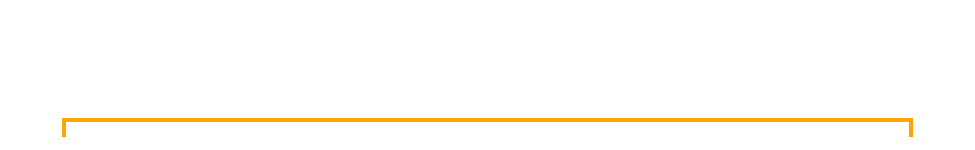
\includegraphics{netsci_files/figure-latex/unnamed-chunk-41-1.pdf}

Okay, let's label both \(1,000\) and \(100,000\) in the above number line:

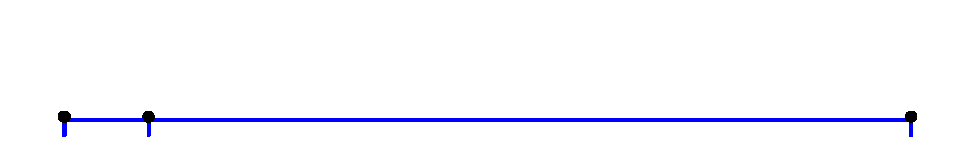
\includegraphics{netsci_files/figure-latex/unnamed-chunk-42-1.pdf}

I plotted four points: 0, 1000, 100000, and 1000000, but can only see three. Why? It's because 0 and 1000 are almost at the same place. But I guess you've probably thought \(1,000\) was in the place of \(100,000\), right?

You can learn some basics of \textbf{log scale} by watching \href{https://www.youtube.com/watch?v=sBhEi4L91Sg}{this video} by Khan Academy.

One of the reasons why people need log scale is that it allows us to include a much wider range of numbers in limited space. For example, it is useful \href{https://www.youtube.com/watch?v=RFn-IGlayAg}{when we measure earthquakes}.

\hypertarget{properties-of-power-law-distributions}{%
\subsection{Properties of power-law distributions}\label{properties-of-power-law-distributions}}

\hypertarget{porperty-1-a-fat-tail-allowing-for-many-outliers}{%
\subsubsection{Porperty 1: A fat tail allowing for many outliers}\label{porperty-1-a-fat-tail-allowing-for-many-outliers}}

\begin{rmdnote}
The following came from the online course of \href{https://github.com/yy/netsci-course}{INFO 606} at Indiana University taught by Professor \href{https://yongyeol.com/}{Yong-Yoel (``YY'') Ahn}.
\end{rmdnote}

A power-law distribution can be expressed as

\begin{equation} 
  p(x) = Cx^{-\lambda} \label{eq:power-law}
\end{equation}

where \(\lambda\) \textgreater{} 1 \footnote{Read here for why: \url{http://tuvalu.santafe.edu/~aaronc/courses/7000/csci7000-001_2011_L2.pdf}.}.

If we take a logarithm of Eq. \eqref{eq:power-law}, we'll have

\begin{align} 
  \ln p(x) & =  \ln (Cx^{-\lambda}) \\
  & = \ln C -\lambda \ln x \label{eq:power-law-simplified}
\end{align}

If you are not familiar with \(\ln\) or how the above calculations are done, do read \href{https://www.math10.com/en/algebra/logarithm-log-ln-lg.html}{this tutorial} on logarithm.

\begin{rmdtip}
If \(a^b=c\), then, \(\log_a c =b\), where \(c>0\), \(a>0\), and \(a \neq 1\). In this example, \(a\) is called \textbf{base} of the logarithm.

\begin{itemize}
\tightlist
\item
  If the \textbf{base} is \(10\): \(\log_{10} a\) will be denoted as \emph{\(\lg a\)}
\item
  If the \textbf{base} is \(e\): \(\log_e a\) will be denoted as \emph{\(\ln a\)}
\end{itemize}

Some logarithmic identities:

\begin{enumerate}
\def\labelenumi{\arabic{enumi}.}
\tightlist
\item
  \(log_a b^c = c \cdot log_a b\);
\item
  \(log_a {b \cdot c} = log_a b + log_a c\);
\item
  \(log_a \frac{b}{c} = log_a b - log_a c\);
\item
  \(log_a^c b = \frac{1}{n} \cdot log_a b\)
\end{enumerate}
\end{rmdtip}

Since \(\ln C\) is a constant, what we get is basically \textbf{a linear function}.
To better understand it, let's plot it.

Before we take the log:

\begin{Shaded}
\begin{Highlighting}[]
\NormalTok{x }\OtherTok{\textless{}{-}} \DecValTok{1}\SpecialCharTok{:}\DecValTok{100}
\NormalTok{y }\OtherTok{\textless{}{-}} \DecValTok{5}\SpecialCharTok{*}\NormalTok{x}\SpecialCharTok{\^{}}\NormalTok{(}\SpecialCharTok{{-}}\DecValTok{2}\NormalTok{)}
\FunctionTok{plot}\NormalTok{ (x, y, }\AttributeTok{pch=}\DecValTok{19}\NormalTok{, }\AttributeTok{cex=}\FloatTok{0.5}\NormalTok{, }\AttributeTok{col=}\StringTok{"orange"}\NormalTok{,}
      \AttributeTok{xlab=}\StringTok{"X"}\NormalTok{, }\AttributeTok{ylab=}\StringTok{"5*x\^{}({-}2)"}\NormalTok{,}
      \AttributeTok{main=}\StringTok{"Before taking a log"}\NormalTok{)}
\end{Highlighting}
\end{Shaded}

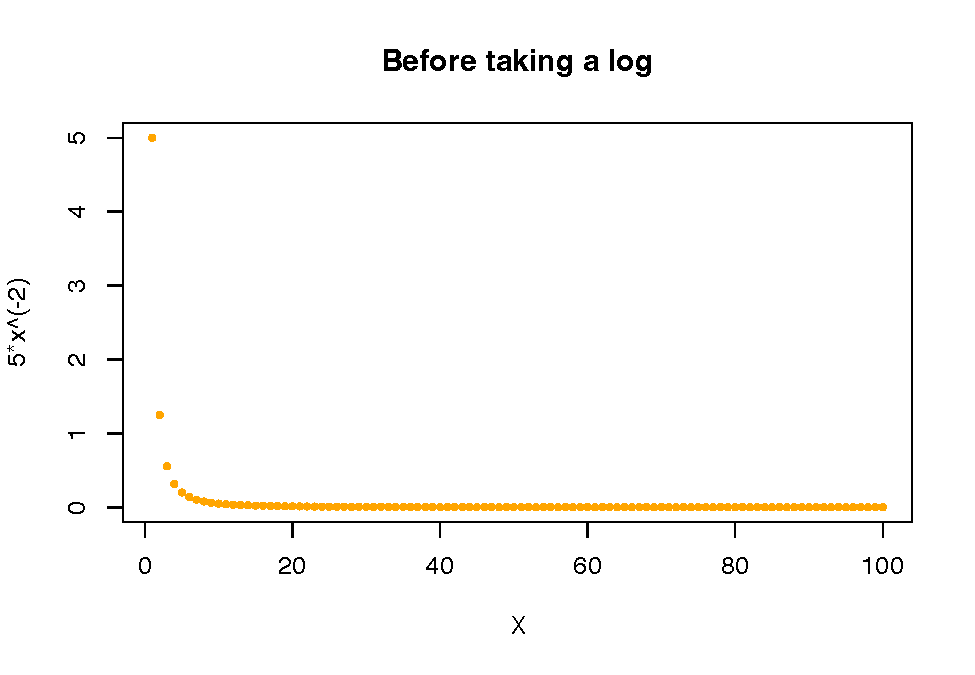
\includegraphics{netsci_files/figure-latex/unnamed-chunk-45-1.pdf}

I learned a lot about how to style the points from reading \href{https://kateto.net/networks-r-igraph}{Dr.Katya Ognyanova's blog post}.

If we take a log:

\begin{Shaded}
\begin{Highlighting}[]
\NormalTok{x }\OtherTok{\textless{}{-}} \DecValTok{1}\SpecialCharTok{:}\DecValTok{100}
\NormalTok{y }\OtherTok{\textless{}{-}} \DecValTok{5}\SpecialCharTok{*}\NormalTok{x}\SpecialCharTok{\^{}}\NormalTok{(}\SpecialCharTok{{-}}\DecValTok{2}\NormalTok{)}
\FunctionTok{plot}\NormalTok{ (x, y, }\AttributeTok{pch=}\DecValTok{19}\NormalTok{, }\AttributeTok{cex=}\FloatTok{0.5}\NormalTok{, }\AttributeTok{col=}\StringTok{"orange"}\NormalTok{,}
      \AttributeTok{xlab=}\StringTok{"log(X)"}\NormalTok{, }\AttributeTok{ylab=}\StringTok{"log(Y)"}\NormalTok{,}
      \AttributeTok{main=}\StringTok{"After taking a log"}\NormalTok{,}
      \AttributeTok{log=}\StringTok{"xy"}
\NormalTok{      )}
\end{Highlighting}
\end{Shaded}

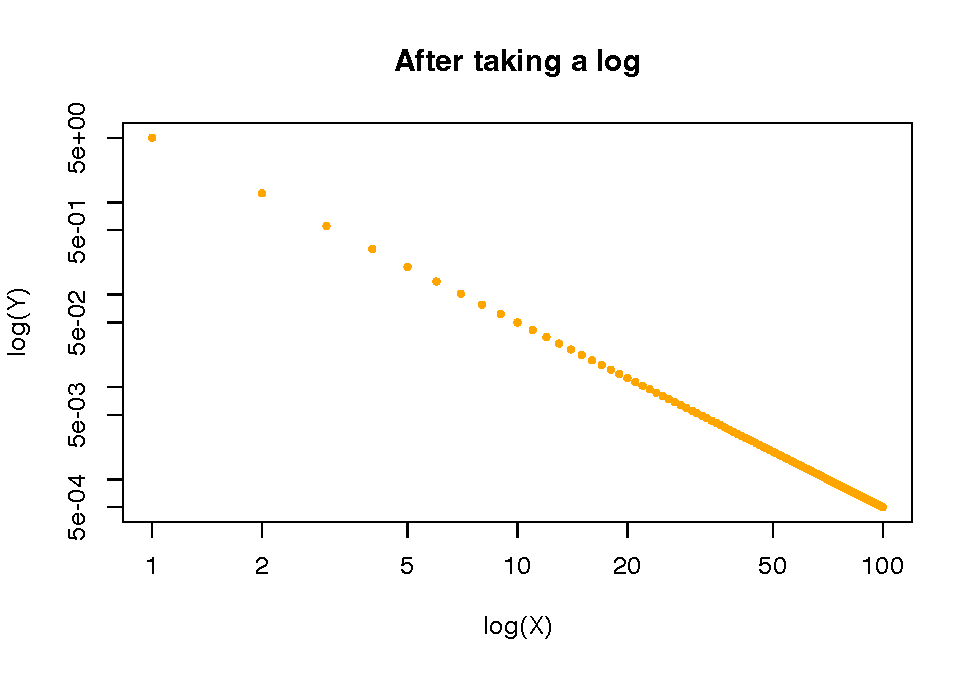
\includegraphics{netsci_files/figure-latex/unnamed-chunk-46-1.pdf}

A very important property of power-law distribution on a log-log scale is it has a \textbf{heavy tail} or a so-called \textbf{fat tail}. Lots of other distributions, like binomial, Poisson, or normal distributions, simply do not have this fat tail, which is super useful when we have lots of outliers in the tail of the distribution.

As we can clearly see below, except for the power-law distribution on a log-log scale, in all the three other distributions, \(y\) quickly reaches zero:

\begin{Shaded}
\begin{Highlighting}[]
\FunctionTok{par}\NormalTok{(}\AttributeTok{mfrow=}\FunctionTok{c}\NormalTok{(}\DecValTok{2}\NormalTok{,}\DecValTok{2}\NormalTok{))}
\CommentTok{\# The idea of the following codes comes from}
\CommentTok{\# https://www.statology.org/plot{-}normal{-}distribution{-}r/}
\NormalTok{x\_dnorm }\OtherTok{\textless{}{-}} \FunctionTok{seq}\NormalTok{(}\SpecialCharTok{{-}}\DecValTok{6}\NormalTok{, }\DecValTok{6}\NormalTok{, }\AttributeTok{length=}\DecValTok{100}\NormalTok{)}
\NormalTok{y\_dnorm }\OtherTok{\textless{}{-}} \FunctionTok{dnorm}\NormalTok{(x\_dnorm)}
\FunctionTok{plot}\NormalTok{(x\_dnorm, y\_dnorm, }\AttributeTok{pch=}\DecValTok{19}\NormalTok{, }\AttributeTok{cex=}\FloatTok{0.5}\NormalTok{, }\AttributeTok{col=}\StringTok{"skyblue"}\NormalTok{,}
     \AttributeTok{main=}\StringTok{"Normal Distribution"}\NormalTok{)}
\CommentTok{\# The following codes are from }
\CommentTok{\# https://www.tutorialspoint.com/r/r\_binomial\_distribution.htm}
\NormalTok{x\_dbinom }\OtherTok{\textless{}{-}} \FunctionTok{seq}\NormalTok{(}\DecValTok{0}\NormalTok{,}\DecValTok{50}\NormalTok{,}\AttributeTok{by =} \DecValTok{1}\NormalTok{)}
\NormalTok{y\_dbinom }\OtherTok{\textless{}{-}} \FunctionTok{dbinom}\NormalTok{(x\_dbinom,}\DecValTok{50}\NormalTok{,}\FloatTok{0.5}\NormalTok{)}
\FunctionTok{plot}\NormalTok{(x\_dbinom, y\_dbinom, }\AttributeTok{pch=}\DecValTok{19}\NormalTok{, }\AttributeTok{cex=}\FloatTok{0.5}\NormalTok{, }\AttributeTok{col=}\StringTok{"red"}\NormalTok{,}
     \AttributeTok{main =} \StringTok{"Binomail Distribution"}\NormalTok{)}
\CommentTok{\# The following codes are from https://statisticsglobe.com/poisson{-}}
\CommentTok{\# distribution{-}in{-}r{-}dpois{-}ppois{-}qpois{-}rpois}
\NormalTok{x\_dpois }\OtherTok{\textless{}{-}} \FunctionTok{seq}\NormalTok{(}\SpecialCharTok{{-}}\DecValTok{5}\NormalTok{, }\DecValTok{50}\NormalTok{, }\AttributeTok{by =} \DecValTok{1}\NormalTok{)}
\NormalTok{y\_dpois }\OtherTok{\textless{}{-}} \FunctionTok{dpois}\NormalTok{(x\_dpois, }\AttributeTok{lambda =} \DecValTok{10}\NormalTok{)}
\FunctionTok{plot}\NormalTok{(x\_dpois, y\_dpois, }\AttributeTok{pch=}\DecValTok{19}\NormalTok{, }\AttributeTok{cex=}\FloatTok{0.5}\NormalTok{, }\AttributeTok{col=}\StringTok{"purple"}\NormalTok{,}
     \AttributeTok{main =} \StringTok{"Poisson Distribution"}\NormalTok{)}
\NormalTok{x }\OtherTok{\textless{}{-}} \DecValTok{1}\SpecialCharTok{:}\DecValTok{100}
\NormalTok{y }\OtherTok{\textless{}{-}} \DecValTok{5}\SpecialCharTok{*}\NormalTok{x}\SpecialCharTok{\^{}}\NormalTok{(}\SpecialCharTok{{-}}\DecValTok{2}\NormalTok{)}
\FunctionTok{plot}\NormalTok{ (x, y, }\AttributeTok{pch=}\DecValTok{19}\NormalTok{, }\AttributeTok{cex=}\FloatTok{0.5}\NormalTok{, }\AttributeTok{col=}\StringTok{"orange"}\NormalTok{,}
      \AttributeTok{xlab=}\StringTok{"log(X)"}\NormalTok{, }\AttributeTok{ylab=}\StringTok{"log(Y)"}\NormalTok{,}
      \AttributeTok{main=}\StringTok{"Power{-}law Distribution (Log{-}Log Scale)"}\NormalTok{,}
      \AttributeTok{log=}\StringTok{"xy"}\NormalTok{)}
\end{Highlighting}
\end{Shaded}

\begin{figure}

{\centering 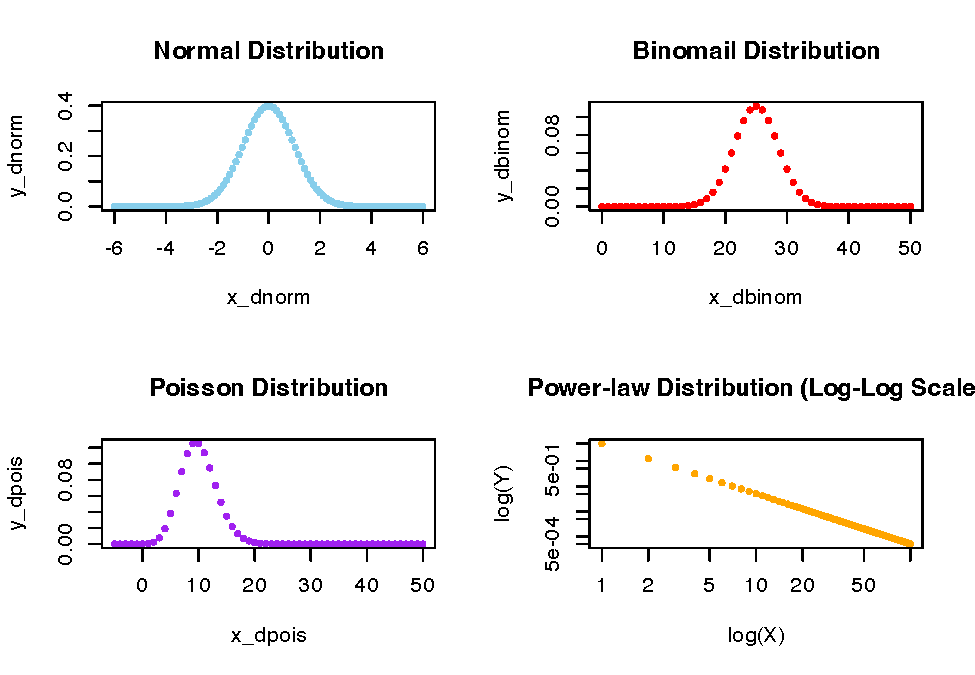
\includegraphics[width=1\linewidth]{netsci_files/figure-latex/unnamed-chunk-47-1} 

}

\caption{Comparing Four Different Distributions}\label{fig:unnamed-chunk-47}
\end{figure}

If we have many outliers in the tail, for example, in the household income distribution shown below by \citet{donovan2016us}, which of the four distributions shown above will you choose to fit the income distribution? Definitely we'll use the power-law distribution which has a fat tail.

\begin{figure}

{\centering \includegraphics[width=0.9\linewidth]{images/income_distribution} 

}

\caption{US Household Income Distribution in 2015, Visualization by @donovan2016us}\label{fig:unnamed-chunk-48}
\end{figure}

We can also compare a normal distribution and a power-law distribution side by side:

\begin{Shaded}
\begin{Highlighting}[]
\FunctionTok{par}\NormalTok{(}\AttributeTok{mfrow=}\FunctionTok{c}\NormalTok{(}\DecValTok{2}\NormalTok{,}\DecValTok{1}\NormalTok{))}
\NormalTok{x\_dnorm\_2 }\OtherTok{\textless{}{-}} \FunctionTok{seq}\NormalTok{ (}\DecValTok{0}\NormalTok{, }\DecValTok{10000}\NormalTok{, }\AttributeTok{by =} \DecValTok{1}\NormalTok{)}
\NormalTok{y\_dnorm\_2 }\OtherTok{\textless{}{-}}\FunctionTok{dnorm}\NormalTok{(x\_dnorm\_2)}
\FunctionTok{plot}\NormalTok{ (x\_dnorm\_2, y\_dnorm\_2, }\AttributeTok{pch=}\DecValTok{19}\NormalTok{, }\AttributeTok{cex=}\FloatTok{0.1}\NormalTok{, }\AttributeTok{col=}\StringTok{"blue"}\NormalTok{,}
      \AttributeTok{xlab=}\StringTok{"x\_dnorm"}\NormalTok{, }\AttributeTok{ylab=}\StringTok{"y\_dnorm"}\NormalTok{,}
      \AttributeTok{main=}\StringTok{"Normal Distribution"}\NormalTok{)}
\NormalTok{x }\OtherTok{\textless{}{-}} \DecValTok{0}\SpecialCharTok{:}\DecValTok{10000}
\NormalTok{y }\OtherTok{\textless{}{-}} \DecValTok{5}\SpecialCharTok{*}\NormalTok{x}\SpecialCharTok{\^{}}\NormalTok{(}\SpecialCharTok{{-}}\DecValTok{2}\NormalTok{)}
\FunctionTok{plot}\NormalTok{ (x, y, }\AttributeTok{pch=}\DecValTok{19}\NormalTok{, }\AttributeTok{cex=}\FloatTok{0.1}\NormalTok{, }\AttributeTok{col=}\StringTok{"orange"}\NormalTok{,}
      \AttributeTok{xlab=}\StringTok{"log(X)"}\NormalTok{, }\AttributeTok{ylab=}\StringTok{"log(Y)"}\NormalTok{,}
      \AttributeTok{main=}\StringTok{"Power{-}law Distribution (Log{-}Log Scale)"}\NormalTok{,}
      \AttributeTok{log=}\StringTok{"xy"}\NormalTok{)}
\end{Highlighting}
\end{Shaded}

\begin{figure}

{\centering 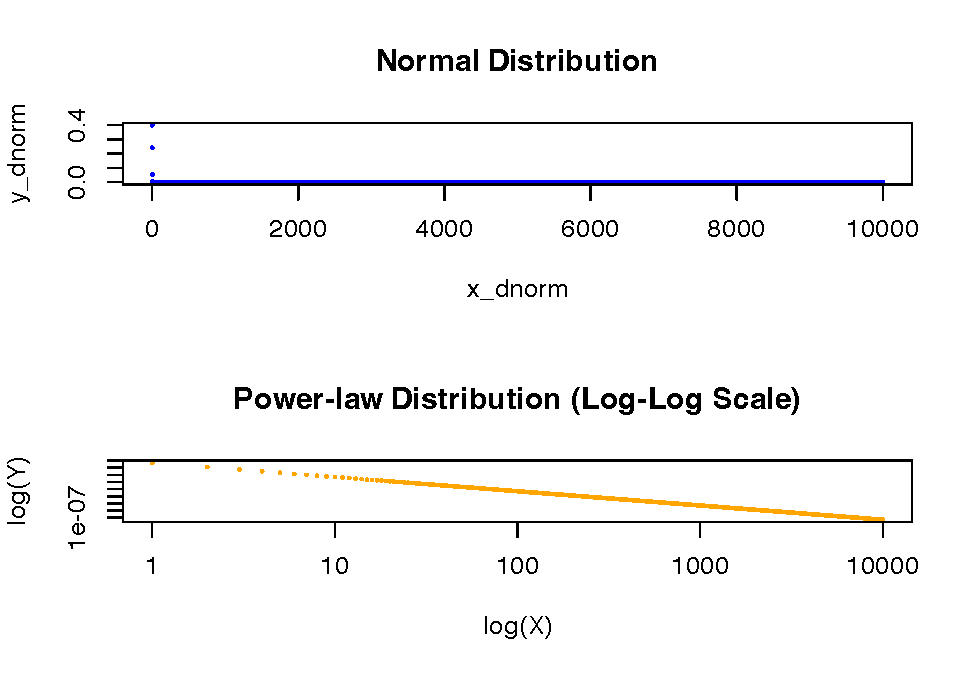
\includegraphics[width=1\linewidth]{netsci_files/figure-latex/unnamed-chunk-49-1} 

}

\caption{Comparing Normal Distribution and Power-law Distribution Side by Side}\label{fig:unnamed-chunk-49}
\end{figure}

In power-law distribution plotted on a log-log scale, we do expect a lot of outliers.

\begin{rmdreminder}
One thing I still did not understand is the range of \(x\). Should it always be \(\ge 1\), or \(\ge 0\)? Why or why not?
\end{rmdreminder}

\hypertarget{property-2-scale-freeness}{%
\paragraph{Property 2: scale-freeness}\label{property-2-scale-freeness}}

To deeply understand what the term ``scale-free'' means, you can read \href{http://networksciencebook.com/chapter/4\#scale-free}{Chapter 4.4} in \href{http://networksciencebook.com/}{Network Science}.

I'll explain in my own words here. To understand ``scale-free'', we must first understand ``scale''. Mark \citet{newman2005power} defines it this way: A scale is ``a typical value around which individual elements are centered (p.1). Therefore, \textbf{scale-free} means that we don't know around \textbf{which} value individual elements in the distribution are centered. A normal distribution is \textbf{not} scale-free because we expect that more than 99\% of the data falls within three standard deviations from the mean.

You can read \href{https://arxiv.org/pdf/cond-mat/0412004.pdf}{\emph{Power laws, Pareto distributions and Zipf's law}} by Mark \citet{newman2005power} for details. This paper is also a must read if you want to gain a deeper understanding about power law.)

In a power-law distribution, it's totally different. For example, if we have \(y = 5 \cdot x^{-2}\). Let's imagine that human height follows this distribution. Suppose your height is \(x\), and \(n\) people have the same height as you. Then you'll see \(\frac{1}{4} \cdot n\) people twice as tall as you\footnote{Just input \(2x\) in the above formula.}, and \(4 \cdot n\) people half of your size. The thing is, \textbf{you don't know where you are located in the distribution!} You can be as tiny as \(10\) inches or as tall as \(100\) feet. Wherever you stand, you will always find \(\frac{1}{4} \cdot n\) people twice as tall as you, and \(4 \cdot n\) people half of your size. \textbf{Think about it!} What a crazy world! That's why we call it \textbf{scale-free}: no inherent scale in the distribution.

\hypertarget{scale-free-property}{%
\section{Scale-free property}\label{scale-free-property}}

\begin{rmdnote}
The following is not originally from me, but my notes from reading \href{http://networksciencebook.com/}{\emph{Network Science}} (Ch. 4.1-4.2) by \href{https://barabasi.com/}{Albert-László Barabási}. Notes are accompanied by my explanations.
\end{rmdnote}

\begin{itemize}
\item
  In real networks, there are hubs that are forbidden in random networks.
\item
  No matter what properties of a network we are studying, we need to base our understanding on the network's \textbf{degree distribution}.
\end{itemize}

The book compares the Poisson distribution and power-law distribution by drawing the degree distribution of the WWW. I wanted to understand these two distributions better so I decided to try drawing them by myself.

The data I used is called \href{http://www-personal.umich.edu/~mejn/netdata/as-22july06.zip}{``Internet''} from \url{http://www-personal.umich.edu/~mejn/netdata/}. I'll use R to plot it. See the result in Figure \ref{fig:powerLaw-poisson}

\begin{Shaded}
\begin{Highlighting}[]
\FunctionTok{library}\NormalTok{(here)}
\NormalTok{internet }\OtherTok{\textless{}{-}} \FunctionTok{read\_graph}\NormalTok{(}\FunctionTok{here}\NormalTok{(}\StringTok{"data"}\NormalTok{,}\StringTok{"as{-}22july06.gml"}\NormalTok{), }
                       \AttributeTok{format =} \StringTok{"gml"}\NormalTok{)}
\CommentTok{\# vcount(internet) \# Getting an idea of its size // 22963}
\NormalTok{deg\_internet }\OtherTok{\textless{}{-}} \FunctionTok{degree}\NormalTok{(internet)}
\CommentTok{\# mean(deg\_internet) \# Calculating average degree // 4.218613}
\NormalTok{x }\OtherTok{\textless{}{-}} \DecValTok{0}\SpecialCharTok{:}\FunctionTok{max}\NormalTok{(deg\_internet) }\CommentTok{\# Setting X{-}axis}
\NormalTok{deg.dist\_internet }\OtherTok{\textless{}{-}} \FunctionTok{degree\_distribution}\NormalTok{(internet, }
                                         \AttributeTok{cumulative =} \ConstantTok{TRUE}\NormalTok{, }
                                         \AttributeTok{mode =} \StringTok{"all"}\NormalTok{)}
\CommentTok{\# This will be the degree distribution of our dataset:}
\NormalTok{y1 }\OtherTok{\textless{}{-}}\NormalTok{ deg.dist\_internet }
\NormalTok{y2 }\OtherTok{\textless{}{-}} \FunctionTok{dpois}\NormalTok{(x, }\AttributeTok{lambda =} \FunctionTok{mean}\NormalTok{(deg\_internet))}
\CommentTok{\# This is to prevent scientific notation on the axes:}
\FunctionTok{options}\NormalTok{(}\AttributeTok{scipen =} \DecValTok{5}\NormalTok{) }
\FunctionTok{plot}\NormalTok{( x, y1, }\AttributeTok{pch=}\DecValTok{19}\NormalTok{, }\AttributeTok{cex=}\FloatTok{0.5}\NormalTok{, }
      \AttributeTok{col=}\StringTok{"orange"}\NormalTok{,}
      \AttributeTok{xlab=}\StringTok{"Degree(log)"}\NormalTok{, }
      \AttributeTok{ylab=}\StringTok{"Probability(log)"}\NormalTok{,}
      \AttributeTok{log =} \StringTok{"xy"}
\NormalTok{      )}
\CommentTok{\# par(new=TRUE) }
\FunctionTok{points}\NormalTok{(x, y2, }\AttributeTok{pch=}\DecValTok{19}\NormalTok{,}
     \AttributeTok{cex=}\FloatTok{0.5}\NormalTok{,}
     \CommentTok{\# log = "xy", \# We can, in fact, do without this line }
     \CommentTok{\# because the above plot is already on a log{-}log scale.}
     \AttributeTok{col=}\StringTok{"blue"}\NormalTok{,}
     \AttributeTok{xlab =} \StringTok{""}\NormalTok{, }
     \AttributeTok{ylab =} \StringTok{""}
\NormalTok{     )}
\end{Highlighting}
\end{Shaded}

\begin{figure}

{\centering 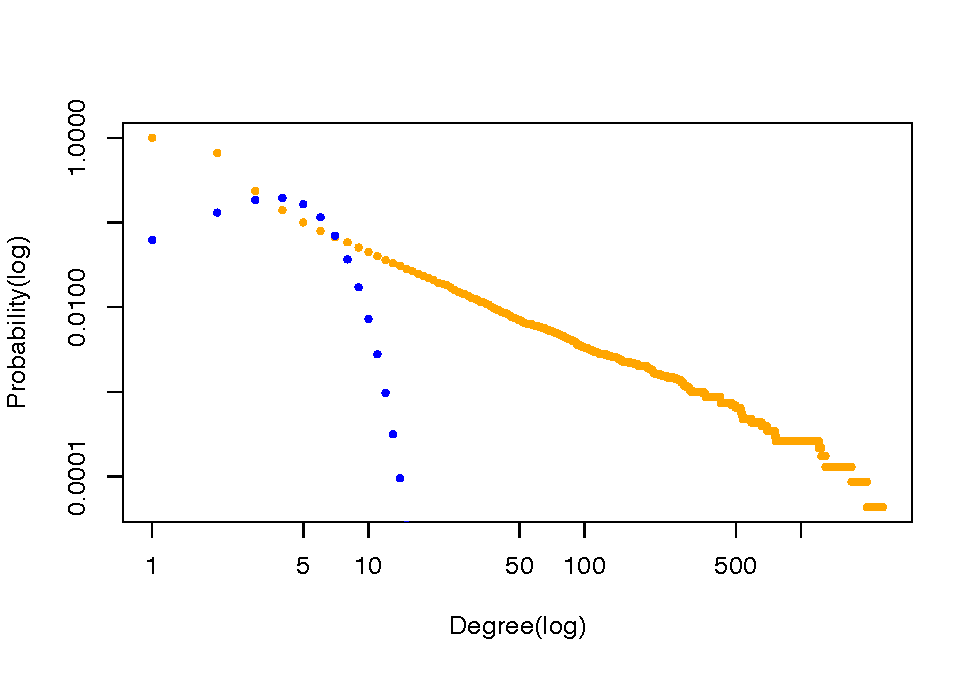
\includegraphics{netsci_files/figure-latex/powerLaw-poisson-1} 

}

\caption{Poisson distribution does not explain degree distribution in real networks}\label{fig:powerLaw-poisson}
\end{figure}

The above code is based on \href{https://stackoverflow.com/questions/6853204/plotting-multiple-curves-same-graph-and-same-scale}{this post}.

We can see that the degree distribution of the real network is different from Poisson distribution but rather roughly follows a power law. We call networks like this as \textbf{scale-free networks}.

A quick note: in the above codes, \texttt{y2\ \textless{}-\ dpois(x,\ lambda\ =\ mean(deg\_internet))} ensures that both networks share the same \(\langle k \rangle\). Therefore, the result in the figure tells us that the degree distribution of this real network cannot be approximated by Poisson distribution.

\hypertarget{hubs}{%
\subsection{Hubs}\label{hubs}}

\begin{rmdnote}
The following is not originally from me, but my notes from reading \href{http://networksciencebook.com/}{\emph{Network Science}} (Ch. 4.3 - 4.7) by \href{https://barabasi.com/}{Albert-László Barabási}. Notes may be accompanied by my explanation.
\end{rmdnote}

Hubs are nodes with high degrees. To understand that there are more hubs in scale-free networks than in random networks, we can refer to Figure \ref{fig:powerLaw-poisson}. The two distributions have exactly the same average degree, \(4.22\).

We will find that compared to random networks, scale-free networks have more low-degree nodes and high-degree nodes, but fewer nodes with degrees near the average degree. This tells us that in random networks, most nodes have comparable degrees (around the average degree of the network) whereas in scale-free networks, there are so many nodes with extremely low and extremely high degrees.

Another difference lies in how the maximum degree (denoted as \(k_{max}\) ) changes as the size of networks increases. For both types of networks, \(k_{max}\) grows as \(N\) becomes larger. The difference is that \(k_{max}\) grows faster (\href{https://en.wikipedia.org/wiki/Polynomial}{polynomially}) with \(N\) in scale-free networks but it grows slower (\href{https://en.wikipedia.org/wiki/Logarithmic_growth}{logarithmatically}) in random networks. Also, if a random network and a scale-free network has the same average degree \(\langle k \rangle\), the \(k_{max}\) in the scale-free network is almost always larger than that in the random network.

Read the section of \emph{The Largest Hub} in \href{http://networksciencebook.com/chapter/4\#hubs}{Chapter 4.3} for formula derivation. I am currently not capable of doing it.

\hypertarget{universality}{%
\subsection{Universality}\label{universality}}

Both World Wide Web (WWW) and the Internet are networks. WWW is a network of information. Its nodes are documents and its links are URLs. In contrast, the Internet is a network of infrastructure. Its nodes are computers and its links are cables and wireless connections. Although they are different, their degree distribution can be both approximated with a power law, meaning that there are a large amount of high degree nodes (``hubs'') and low degree nodes. In other words, both reveal scale-free properties.

Since scale-free properties are so prevalent, we call scale-free property a universal characteristic for networks.

As ubiquitous as it is, the scale-free property isn't for every networks. Many networks do not share this property, for example, power grid and material networks. Scale-freeness requires that the number of links a node can have is arbitrary, and not systematically constrained. If this requirement is not fulfilled, then hubs are restricted and the network won't show a scale-free property.

\begin{rmdimportant}
Not all scholars agree on the universality of scale-free networks in real life, for example, \emph{\href{https://www.nature.com/articles/s41467-019-08746-5}{Scale-free networks are rare}} by Broido and Caluset (2019). And \href{https://www.barabasilab.com/post/love-is-all-you-need}{here} is the response to this paper from Barabási.
\end{rmdimportant}

\hypertarget{ultra-small-property-and-the-role-of-degree-exponent}{%
\subsection{Ultra-small property, and the role of degree exponent}\label{ultra-small-property-and-the-role-of-degree-exponent}}

Small-world property is the only characteristic in real networks that is well explained by random network models, more specifically, by the Watts-Strogatz model.

\begin{rmdreminder}
I still need to work on these two sections. For now, I will just skip them.
\end{rmdreminder}

\begin{rmdreminder}
Barabási Ch: 4.3-4.7 Reading Quiz needs to be done again!
\end{rmdreminder}

\hypertarget{the-barabuxe1si-albert-model}{%
\section{The Barabási-Albert Model}\label{the-barabuxe1si-albert-model}}

The Barabási-Albert model, or BA model for short, addresses this question: how does a network's degree distribution form a power law?

Two hidden assumptions of the random network model do not hold water in real networks:

\begin{enumerate}
\def\labelenumi{\arabic{enumi}.}
\item
  The random network model assumes that the number of nodes is fixed. In real networks, however, this number continues to grow as new nodes join the network. That is to say, the size of a real network keeps growing.
\item
  The random network model assumes that a link is generated randomly. However, in real networks, new nodes prefer to link to high-degree nodes. This phenomenon is called \textbf{preferential attachment}.
\end{enumerate}

The BA model recognized the coexistence of \textbf{network growth} and \textbf{preferential attachment} in real networks and proposed a method of generating networks with scale-free properties, i.e., hubs, and a degree distribution that follows a power law.

\begin{rmdreminder}
I am wondering: does a power law distribution already implies that there are hubs in the network?
\end{rmdreminder}

We begin with \(m_0\) nodes. Each node's degree is no less than 1. Links between these \(m_0\) nodes are arbitrary.

\begin{enumerate}
\def\labelenumi{\arabic{enumi}.}
\item
  At each timestep, a new node \(i\) with a degree of \(m\) (\(m \le m_0\)) is added to the network.
\item
  The probability that node \(i\) connects to an old node, denoted as node \(j\), is \textbf{proportional} to the old node's degree \(k_j\) \citep{menczer2020first}:
\end{enumerate}

\begin{equation}
  \Pi(i, j) = \frac{k_j}{\sum\limits_l k_l} \label{eq:ba-model}
\end{equation}

The denominator in Eq. \eqref{eq:ba-model} is the sum of all degrees in the old network, so the sum of all these probabilities is equal to one \citep{menczer2020first}.

\begin{rmdtip}
I am not sure whether I can explain why the sum of all these probabilities is equal to one this way: Let us say the probability that node \(i\) will connect to node \(1\) is \(P_1\), to node \(2\), \(P_2\), to node \(3\), \(P_3\) \ldots, if we add these probabilities up, it will (and has to) be equal to one.
\end{rmdtip}

\begin{rmdreminder}
In \citet{menczer2020first}, in Box 5.4, it says that \(m\) here is the average degree of the network. I did not quite understand why.
\end{rmdreminder}

\begin{rmdreminder}
The image 5.4 made me wonder whether my computation of \ref{fig:powerLaw-poisson} was wrong. I will check it later.

Update: Yeah, i was wrong. Originally, when calculating \texttt{deg.dist\_internet}, I set \texttt{cumulative} to be \texttt{FALSE}. This is due to the fact that I did not quite understand power law distribution at that time. I need to set it to be \texttt{TRUE}.
\end{rmdreminder}

\hypertarget{improving-the-ba-model}{%
\subsection{Improving the BA model}\label{improving-the-ba-model}}

\begin{rmdnote}
The following is largely from the online course of \href{https://github.com/yy/netsci-course}{INFO 606} at Indiana University taught by Professor \href{https://yongyeol.com/}{Yong-Yoel (``YY'') Ahn}. My notes are accompanied.
\end{rmdnote}

Suppose you are an incoming node and are about to attach yourself to other nodes. According to Eq. \eqref{eq:ba-model}, you first should calculate all the degree nodes in the existing network and then calculate the proportion of a specific node's degree against the sum of all the degrees. This proportion will be the probability that you will connect to this node.

There is a problem in the first step. You need to know all the nodes before you can get the sum of all degrees. However, this is very difficult. For instance, when you enter a university, and are about to develop a friendship with other people, is it realistic for you to first know how many friends \textbf{EVERY} person at this university has? Probably not.

Is it possible for us to achieve preferential attachment without requiring knowledge about each and every node in the existing network?

Yes. Try this: The incoming node randomly chooses a link from the existing network, then connect to either end of this link. Hubs have more links connecting to it, so it is more likely for this incoming node to connect to a hub. If you have difficulty understanding why so, consider the extreme example of a star graph.

\begin{Shaded}
\begin{Highlighting}[]
\NormalTok{starG }\OtherTok{\textless{}{-}} \FunctionTok{make\_star}\NormalTok{(}\AttributeTok{n =} \DecValTok{12}\NormalTok{, }\AttributeTok{mode =} \StringTok{"undirected"}\NormalTok{, }\AttributeTok{center =} \DecValTok{1}\NormalTok{ )}
\FunctionTok{plot}\NormalTok{ (starG)}
\end{Highlighting}
\end{Shaded}

\begin{figure}

{\centering 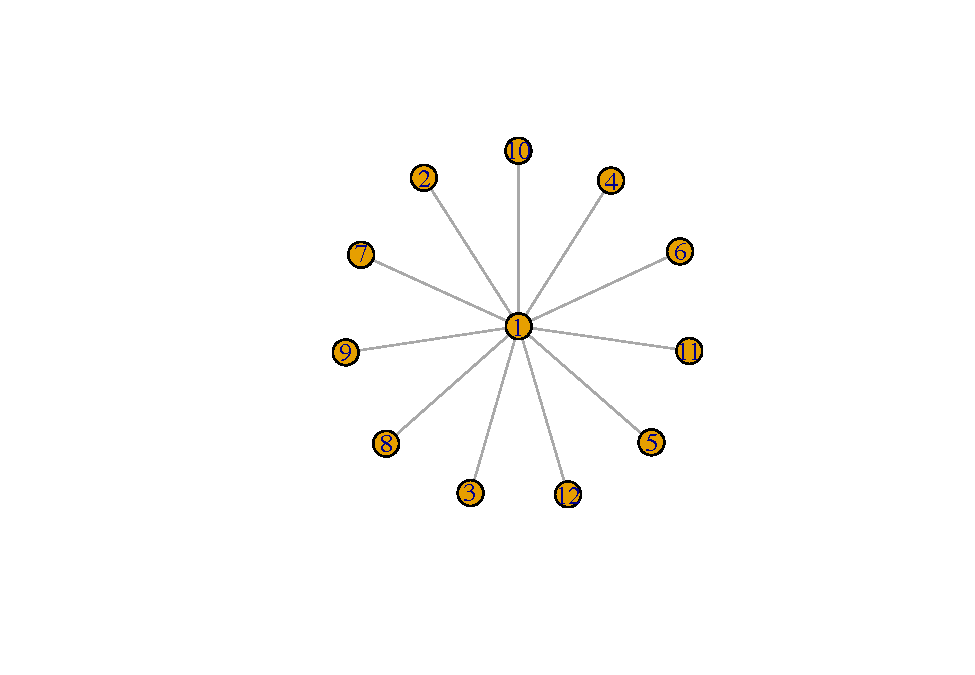
\includegraphics[width=1\linewidth]{netsci_files/figure-latex/starG-1} 

}

\caption{A star graph}\label{fig:starG}
\end{figure}

In Fig. \ref{fig:starG}, no matter which link you pick, it is always connected to the hub.

If you have followed the understood the logic so far, you should be able to know that if \(k_i = 2 \cdot k_j\) (meaning node \(i\) has twice as many links as node \(j\)), then the incoming node is twice as likely to connect to node \(i\). This means that the probability of connecting to node \(i\) is linearly \textbf{proportional} to \(k_i\), which is how the BA model defines preferential attachment.

\begin{rmdreminder}
Professor YY said at the end of the video that this process can also result in a high clustering coeffient of the network. I need to brush up on clustering coeffient a little bit to understand explain why.
\end{rmdreminder}

  \bibliography{book.bib,article.bib}

\backmatter
\printindex

\end{document}
